\documentclass{article}

\usepackage{hyperref}
\usepackage{geometry}
\geometry{left=3cm, right=3cm, bottom=3cm, top=3cm}
\usepackage[section]{placeins}
\usepackage{amsmath}
\usepackage{amsfonts}
\usepackage{amsthm}
\usepackage{dynkin-diagrams}
\usepackage{algorithm2e}
\usepackage{enumerate}
\usepackage{tikz}
\usepackage[outline]{contour}
\contourlength{1.3pt}

% add shell-escape to commands
\usetikzlibrary{knots, cd, external, calc}
\tikzexternalize[prefix=tikz/]

\newtheorem{theorem}{Theorem}[section]
\newtheorem{corollary}[theorem]{Corollary}
\newtheorem{lemma}[theorem]{Lemma}
\newtheorem{proposition}[theorem]{Proposition}
\newtheorem{problem}[theorem]{Problem}
\newtheorem{conjecture}[theorem]{Conjecture}

\theoremstyle{definition}
\newtheorem{examples}[theorem]{Examples}
\newtheorem{example}[theorem]{Example}
\newtheorem{notation}[theorem]{Notation}
\newtheorem{remark}[theorem]{Remark}
\newtheorem{question}[theorem]{Question}
\newtheorem{algo}[theorem]{Procedure}

\newcommand{\coxtwothreethree}{%
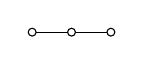
\begin{tikzpicture}[scale=0.5]
\draw (0, 0) circle (0.1);
\draw (1, 0) circle (0.1);
\draw (2, 0) circle (0.1);
\draw (0.1, 0) -- (0.9, 0);
\draw (1.1, 0) -- (1.9, 0);
\end{tikzpicture}}

\newcommand{\coxthreethreethree}{%
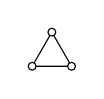
\begin{tikzpicture}[scale = 0.5]
\draw (0, 0) -- (60:1) -- (1, 0) -- (0, 0);
\draw[fill = white] (0, 0) circle (0.1);
\draw[fill = white] (60:1) circle (0.1);
\draw[fill = white] (1, 0) circle (0.1);
\end{tikzpicture}}

\newcommand{\coxthreethreethreetype}[1]{%
\begin{tikzpicture}[scale = 0.5]
\draw (0, 0) -- (60:1) -- (1, 0) -- (0, 0);
\draw[fill = white] (0, 0) circle (0.1);
\draw[fill = white] (60:1) circle (0.1);
\draw[fill = white] (1, 0) circle (0.1);
\node at (0.5, 0.2) {\tiny{#1}};
\end{tikzpicture}}

\newcommand{\coxathreetype}[1]{%
\begin{tikzpicture}[scale=0.5]
\draw (0, 0) circle (0.1);
\draw (1, 0) circle (0.1);
\draw (2, 0) circle (0.1);
\draw (0.1, 0) -- (0.9, 0);
\draw (1.1, 0) -- (1.9, 0);

\node at (0.5, 0.2) {\tiny{#1}};
\end{tikzpicture}}

\newcommand{\coxathreetypedouble}[2]{%
\begin{tikzpicture}[scale=0.5]
\draw (0, 0) circle (0.1);
\draw (1, 0) circle (0.1);
\draw (2, 0) circle (0.1);
\draw (0.1, 0) -- (0.9, 0);
\draw (1.1, 0) -- (1.9, 0);

\node at (0.5, 0.2) {\tiny{#1}};
\node at (1.5, 0.2) {\tiny{#2}};
\end{tikzpicture}}

\newcommand{\coxfourthreethree}{%
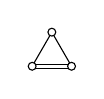
\begin{tikzpicture}[scale = 0.5]
\draw (0, 0) -- (60:1) -- (1, 0);
\draw (0, 0.05) -- (1, 0.05);
\draw (0, -0.05) -- (1, -0.05);
\draw[fill = white] (0, 0) circle (0.1);
\draw[fill = white] (60:1) circle (0.1);
\draw[fill = white] (1, 0) circle (0.1);
\end{tikzpicture}
}

\newcommand{\verticalcenter}[1]{
\begin{tabular}{l} #1 \end{tabular}
}

\begin{document}

\begin{titlepage}
\begin{center}
\pagenumbering{gobble}
\vspace*{1.5cm}
\Large{Department of Mathematics \\ of the University of Bern}\\
\vspace*{3.5cm}
\Huge{\textbf{Coxeter Quotients \\ of Link Groups}}\\
\vspace*{6.5cm}
\Large{Master Thesis of} \\ \Large{\textbf{Levi Ryffel}}\\
\vspace*{.25cm}
Supervised by \\ \textbf{Prof. Dr. Sebastian Baader}\\
\vspace*{2cm}
February 2020
\end{center}
\end{titlepage}
\pagenumbering{arabic}

\tableofcontents
\newpage

\section{Coxeter Groups}
Coxeter groups are of interest for example in geometric group theory, where they form a particularly nice family of examples \cite{davis2008}.
In this thesis we are going to exploit their nice properties and apply them to knot theoretic concepts such as the meridional rank, compare Section \ref{subsec:meridional-rank}.

In this section we are going to introduce the basics of the theory of Coxeter groups, limited to just what we will use afterwards. This is by no means a proper introduction; the reader completely unfamiliar with the theory of Coxeter groups might want to read Chapter 5 from Humphreys' book~\cite{humphreys1990} before reading what follows.

\subsection{Coxeter Matrices and Graphs}
Let $S$ be a finite set and let $M = (m_{st})$ be a symmetric $S \times S$ matrix with coefficients in the set of natural numbers, possibly $\infty$, satisfying $m_{ss} = 1$ for all $s \in S$, and $m_{st} \geq 2$ if $s \ne t$. Such a matrix is called a \textit{Coxeter matrix}. Consider the group presentation
$$W = \langle S \; | \; (st)^{m_{st}} = 1 \text{ for } s,t\in S \rangle,$$
where we do not include relations of the form $(st)^\infty = 1$.
Then the group $W$ is called the \textit{Coxeter group} corresponding to $M$. The tuple $(W,S)$ is called a \textit{Coxeter system} and the cardinality $\#S$ is referred to as its \textit{rank}. Since for us Coxeter groups always arise with a generating set, we blur the distinction between Coxeter groups and Coxeter systems.

Another way to encode the coefficients $m_{st}$ is to use them as weights in weighted undirected graphs, so-called \textit{Coxeter graphs}. In this case, the nodes of the graph associated to $W$ are the generators $S$, and the weight between the nodes $s$ and $t$ is $m_{st}$. The following shorthand notations are very common: If $m_{st} = 2$, then the edge between $s$ and $t$ is omitted. If $m_{st} = 3$, then the weight on the edge between $s$ and $t$ is omitted. Finally, if $m_{st} = 4$ then instead of a labeled line we draw an unlabeled double line.

\begin{example}[Dihedral Groups]
The symmetry group of a regular $n$-gon is called the 
\textit{dihedral group} of order $2n$, denoted by the symbol $D_n$. This group is generated by two reflections 
$s, t$ whose composition is a rotation by an angle 
of~$2\pi/n$. This is used to show that $D_n$ 
is isomorphic to the Coxeter group
$$W = \langle s, t \; | \; (st)^n = s^2 = t^2 = 1 \rangle.$$
Thus, Coxeter groups on two generators whose product has finite order are dihedral groups.

This observation is often used to motivate the introduction of one more dihedral group, the so-called \textit{infinite dihedral group} with presentation
$$D_\infty = \langle s, t \; | \; s^2 = t^2 = 1 \rangle.$$
\end{example}
\subsection{The Reflection Representation}
A well-known construction leading to an easy solution of the word-problem for Coxeter groups and also helping in adapting a geometric viewpoint to the study of Coxeter groups is a faithful representation of any Coxeter group where its generating set acts as a set of reflections with respect to a (possibly degenerate) bilinear form.

Let $(W,S)$ be a Coxeter system. Then we consider the bilinear form on the vector space $V = \mathbb{R}^S$ given by the matrix $B = (b_{st})$ with entries $b_{st} = -\cos \pi/m_{st}$. 
For a generating reflection $s$ in $S$ let $\rho_s$ be the \textit{reflection} with respect to $B$ with root the basis vector~$e_s$ in $\mathbb{R}^S$ given by the formula
$$ \rho_s(x) = x - 2B(x, e_s)e_s,$$
where $x$ is a vector in $V$.

\begin{proposition}\label{prop:reflection-representation-well-defined}
Let $(W,S)$ be a Coxeter system and let $s, t \in S$. Then the reflections $\rho_s$ and $\rho_t$ satisfy $(\rho_s \rho_t)^{m_{st}} = 1$.
\end{proposition}

\begin{proof}
Let $n$ be the number of elements of $S$. Observe that each reflection $\rho_s$ fixes an $(n-1)$-dimensional hyperplane, namely the orthogonal complement of the non-isotropic vector $e_s$. Now fix generating reflections $s$ and $t$ in $S$ and consider the subspace $V_{st} = \mathbb{R}e_s \oplus \mathbb{R}e_t$, which is invariant under the maps $\rho_s$ and $\rho_t$. Since the orthogonal complement of $V_{st}$ is fixed by $\rho_s$ and $\rho_t$, the order of $\rho_s\rho_t$ on $V$ is equal to its order on $V_{st}$.

Let us now distinguish two cases. If $m_{st}$ is finite, $B$ restricted to $V_{st}$ is positive definite. To see this, consider an arbitrary non-zero vector $v = ae_s + b e_t$ in $V_{st}$ and compute
\begin{align*}
B(v, v) & = a^2B(e_s, e_s) + 2abB(e_s, e_t) + b^2B(e_t, e_t)\\
& = a^2 + 2ab\text{cos}( -\pi / m_{st} ) + b^2 \\
& > 0.
\end{align*}
Thus, $V_{st}$ is isometric to $\mathbb{R}^2$ with the standard inner product, and the angle between the invariant subspaces of $\rho_s$ and $\rho_t$ is equal to $2 \pi / m_{st}$. This shows that $\rho_s$ and $\rho_t$ are symmetries of a regular polygon and their product is a rotation by $2\pi/m_{st}$, which has order $m_{st}$.
On the other hand, if $m_{st} = \infty$ the matrix of $\rho_s\rho_t$ is given by
$$\rho_s \rho_t = \left( \begin{matrix}
-1 & 1 \\ 1 & -1
\end{matrix} \right)
\left( \begin{matrix}
1 & -1 \\ -1 & 1
\end{matrix} \right)
= \left( \begin{matrix}
-2 & 2 \\ 2 & -2
\end{matrix} \right)
$$
which has infinite order.
\end{proof}

This shows that the map $s \mapsto \rho_s$ induces a representation of $W$, called the \textit{reflection representation} of $W$. We will conclude this section by showing that this representation is faithful. But first we need some preparation.
To any Coxeter group $W$ we can assign a \textit{length function} $l: W \rightarrow \mathbb{N}$, assigning to any element~$w$ of $W$ the minimal number of generating reflections needed to write down an expression for $w$. An expression for $w$ of length $l(w)$ is called a \textit{reduced expression} for $w$.
To get a little bit of a feeling how the length function behaves for Coxeter groups (or more generally, for groups generated by elements of order two subject only to relations of even length, such as the reflection quotient from Section \ref{subsec:reflection-quotient}), we prove the following illustrative result.

\begin{proposition}
Let $W$ be a Coxeter group, $w \in W$ and $s \in S$. Then $l(ws) = l(w) \pm 1$.
\end{proposition}

\begin{proof}
First of all, we make the observation that for any words 
$w, w' \in W$ we have $l(ww') \leq l(w) + l(w')$. This immediately implies that $l(ww') \geq l(w) - l(w')$ by applying the above to the words $ww'$ and $w'^{-1}$ instead of $w$ and $w'$, observing that $l(w) = l(w^{-1})$ for all $w$ in $W$. We conclude that
$$l(w) - 1 \leq l(ws) \leq l(w) + 1.$$
The only thing left to show is that in fact $l(ws) \neq l(w)$. To see this, we introduce the \textit{sign} homomorphism $\varepsilon: W \rightarrow \{\pm 1\}$ defined via $s \mapsto -1$ for all $s$ in $S$. Indeed, this extends to~$W$ since all relations of~$W$ are of even length. Obviously we have $\varepsilon(w) = (-1)^{l(w)}$, and $\varepsilon(ws) \neq \varepsilon(w)$. Using this, we conclude that $l(ws) \neq l(w)$, which is precisely what we wanted to show.
\end{proof}

For a non-zero vector $v$ in $V$ we will say that $v$ is \textit{positive} if $v$ is a non-negative linear combination of the basis vectors $e_s$. Moreover, $v$ is \textit{negative} if $-v$ is positive. This enables us to formulate the following important Lemma relating the length function to the reflection representation.

\begin{lemma}\label{lem:humphreys5.4}
Let $W$ be a Coxeter group, $w$ be a word in $W$ and $s$ a generating reflection in $S$. Then the vector $we_s$ in $V$ is positive if and only if we have that $l(ws) = l(w) + 1$.
\end{lemma}

\begin{proof}
This is taken from \cite{humphreys1990}. Note first that it suffices to prove that whenever $l(ws) = l(w) + 1$ we have that $we_s$ is positive, since applying this to $ws$ instead of $w$ proves its converse. 
The proof of this implication is a proof by induction on $l(w)$. Suppose $l(w) = 0$. Then $w$ is the identity and we have that $l(ws) = l(w) + 1$ for all $s$. 

For the inductive step, Let $t$ be any reflection in $S$ such that $l(wt) = l(w) - 1$, taking for example~$t$ to be the last symbol in a reduced expression for $w$. Write $w = w'w_{st}$, where $w_{st}$ is a word in the symbols $s, t$ of maximal length such that the length of the expression $w'w_{st}$ is equal to $l(w)$. This exists since $w_{st}$ equal to the empty word is in fact a (non-optimal) solution.
We will now prove the Lemma by showing that the vectors $w'e_s$, $w'e_t$ and $w_{st}e_s$ are all positive, and that $w_{st}$ is non-trivial. Taking $w_{st} = t$ shows that $l(w') < l(w)$, so we can apply the induction hypothesis to $w'$, showing that the vectors $w'e_s$ and $w'e_t$ are both positive, provided we can show $l(w's) > l(w')$ and $l(w't) > l(w')$. 
Suppose toward a contradiction that $l(w's) < l(w')$. Then $sw_{st}$ is in fact a longer word than $w_{st}$, contradicting maximality of $w_{st}$. Similarly it is also true that $l(w't) > l(w')$.


\begin{figure}[ht]
\centering
\begin{minipage}{.5\textwidth}
\centering
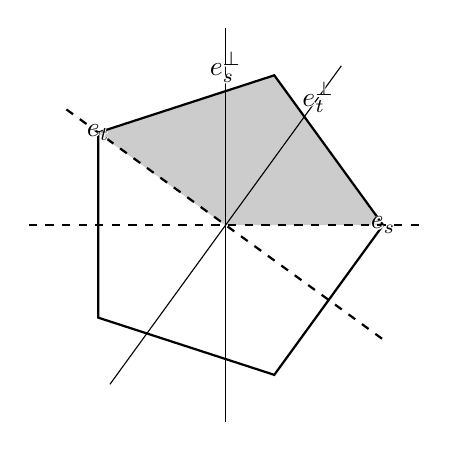
\begin{tikzpicture}[scale = 0.5]
% pentagon
\filldraw[color = black!20] (4, 0) -- (72:4) -- (144:4) -- (0, 0);
\draw[thick] (4, 0) -- (72:4) -- (144:4) -- (216:4) -- (288:4) -- (4, 0);
\draw[thick, dashed] (-5, 0) -- (5, 0);
\draw[thick, dashed] (144:5) -- (144:-5);
\draw (0, -5) -- (0, 5);
\draw (54:5) -- (54:-5);

\node at (4, 0) {\contour{white}{$e_s$}};
\node at (144:4) {\contour{white}{$e_t$}};
\node at (0, 4) {\contour{white}{$e_s^\perp$}};
\node at (54:4) {\contour{white}{$e_t^\perp$}};


\end{tikzpicture}
\end{minipage}%
\begin{minipage}{.5\textwidth}
\centering

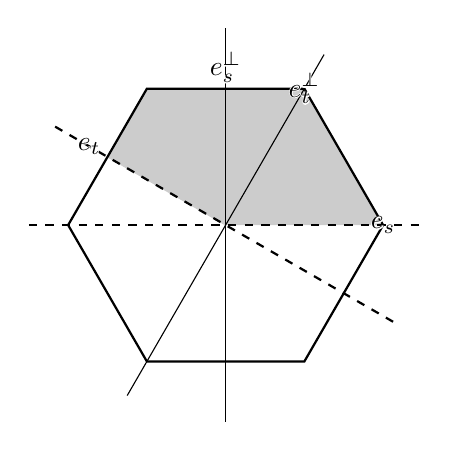
\begin{tikzpicture}[scale = 0.5]
% hexagon
\filldraw[color = black!20] (4, 0) -- (60:4) -- (120:4) -- ($(120:4)!0.5!(180:4)$) -- (0, 0);
\draw[thick] (4, 0) -- (60:4) -- (120:4) -- (180:4) -- (60:-4) -- (120:-4) -- (4, 0);

\draw[thick, dashed] (-5, 0) -- (5, 0);
\draw[thick, dashed] (150:5) -- (150:-5);
\draw (0, -5) -- (0, 5);
\draw (60:5) -- (60:-5);

\node at (4, 0) {\contour{white}{$e_s$}};
\node at (150:4) {\contour{white}{$e_t$}};
\node at (60:4) {\contour{white}{$e_t^{\perp}$}};
\node at (90:4) {\contour{white}{$e_s^\perp$}};

\end{tikzpicture}
\end{minipage}
\caption{Illustration of the fact that $e_s$ lands in the positive cone, indicated in grey. Note that composing reflections in the mirrors $e_s^\perp$ and $e_t^\perp$ results in a rotation by an angle of $2\pi/m_{st}$.}
\label{fig:humphreys-5.4-proof}
\end{figure}

Finally we draw a picture to show that $v_{st}e_s$ is positive. Note first that $v_{st}$ does not have a reduced expression ending in $s$, since if it did we would actually reduce its length by adding an $s$ to the end. In particular, the length of $w_{st}$ is strictly less than $m_{st}$, that is, interpreting $w_{st}$ as a map on the plane as in the proof of Proposition \ref{prop:reflection-representation-well-defined}, $w_{st}$ is not rotation by an angle of $\pi$. The claim now follows from the fact that $w_{st}$ is a rotation by at most $\pi - \pi/m$, perhaps followed by a reflection in $e_t^\perp$, but only if this does not result in a rotation by an angle of~$\pi$. Also compare Figure \ref{fig:humphreys-5.4-proof}.
\end{proof}

Having established how the length function is related to the action of $W$ on the basis vectors of its geometric representation, we immediately obtain what we desired.

\begin{theorem}
The reflection representation is faithful.
\end{theorem}

\begin{proof}
Suppose $w$ lies in the kernel of the reflection representation. Then obviously $we_s > 0$ for all generating reflections $s$ in $S$, so by Lemma \ref{lem:humphreys5.4}, $l(ws) = l(w) + 1$ for all $s$. That is, for any $s$ we have that $w$ does not have a reduced expression ending in $s$. But this implies that $w$ is the identity.
\end{proof}

\subsection{Roots}\label{subsec:roots}
The main goal of this section is to show that Coxeter groups have tiny center, that is, the center of an infinite Coxeter group is trivial. To do this, our main tool will be the action of a Coxeter group on a specific subset of $V$ called roots.

The set of \textit{roots} of a Coxeter group $W$, denoted by the letter $\Phi$, is the set of all images of the basis vectors $e_s$ under $W$. The geometric observation justifying this terminology is the following. Let $w$ be an arbitrary element of $W$. Then, for all generating reflections $s$ in $S$, the map $wsw^{-1}$ acts on $V$ by a reflection whose eigenvector of eigenvalue one is the vector $we_s$.

Note that by Lemma \ref{lem:humphreys5.4}, every root is either positive or negative. Writing $\Pi$ for the set of positive roots, we can express this in symbols as $\Phi = \Pi \cup -\Pi$. This will be useful for a geometric characterization of the length function $l$ on a Coxeter group. Consider the function $n$ mapping an element $w \in W$ to the number of positive roots sent to negative roots by the action of $w$ on $V$.

\begin{proposition}\label{prop:n=l}
Let $W$ be a Coxeter group. Then, for any element $w$ of $W$ we have that $n(w) = l(w)$.
\end{proposition}

\begin{proof}
Let $s$ be a generating reflection in $S$. We first prove that the only positive root mapped to a negative root by $s$ is the basis vector $e_s$. Choose any positive root $\alpha \neq e_s$. Since $\alpha$ is not equal to $e_s$ there exists a reflection $t$ in $S$ such that the coefficient of $\alpha$ corresponding to the $e_t$-component of $\alpha$ is non-zero. But the reflection $s$ does not change the $e_t$-component of $\alpha$, so $s\alpha$ must be positive.

We now proceed by induction on the number $l(w)$. Suppose $l(ws) > l(w)$, and that $n(w) = l(w)$. By Lemma \ref{lem:humphreys5.4} it follows that $we_s$ is positive, which shows that $wse_s = -we_s$ is negative. Note that since $w$ induces a bijection on the remaining positive roots $\Pi \setminus \{e_s\}$, we must have $n(ws) = n(w) + 1 = l(ws)$.
\end{proof}

Recall that the \textit{radical} $V^\perp$ of the bilinear form $B$ on $V$ is the set of vectors~$v'$ in $V$ such that we have $B(v, v') = 0$ for all $v$ in $V$. Note that $V^\perp$ is not affected by any reflection, so in particular $V^\perp$ is a $W$-invariant subspace. We will now prove a partial converse to this for \textit{irreducible} Coxeter groups, that is, Coxeter groups whose associated Coxeter graph is connected.

\begin{theorem}\label{thm:invariant-subspaces}
Let $W$ be an irreducible Coxeter group. Then, every proper $W$-invariant subspace of~$V$ is contained in $V^\perp$.
\end{theorem}

\begin{proof}
Let $V'$ be a $W$-invariant subspace of $V$. Suppose first that some basis vector $e_s$ is contained in~$V'$. Let $t$ be adjacent to $s$ in the Coxeter graph of $W$. Then $te_s$ has a non-zero $e_t$-component and is contained in $V'$, so it follows that also $e_t$ is in $V'$. Proceeding like this through the connected Coxeter graph of $W$ we obtain that $V'$ contains a basis of $V$. Therefore, $V'$ is not a proper subspace.

We have established that all proper $W$-invariant subspaces of $V$ do not contain any basis vectors~$e_s$. Let $V'$ be such a subspace. Then $V'$ is contained in an intersection of eigenspaces of the generating reflections $s$ in $S$. But since the proper subspace $V'$ does not contain the basis vectors~$e_s$, we have that~$V'$ must be contained in the eigenspaces of $s$ in $S$ of eigenvalue $1$, in other words, in the orthogonal complements of the basis vectors $e_s$.
\end{proof}

\begin{corollary}
The center of an infinite Coxeter group is trivial.
\end{corollary}

\begin{proof}
Let $A$ be any endomorphism of $V$ commuting with every element of $W$. We will show that $A$ is actually multiplication with a scalar. Let $s \in S$ be any generating reflection. Since $A$ commutes with $s$ their eigenspaces must agree. In particular, the line $\mathbb{R}e_s$ is an eigenspace of $A$ of eigenvalue $c$ for some $c$. 

Let $V'$ be the kernel of the map $A-c$. Let $v \in V'$. Then $Av = cv$. But then we have
\begin{align*}
(A-c)wv & = Awv - cwv \\
& = wAv - cwv \\
& = w(A - c) v \\
& = 0,
\end{align*}
so $V'$ is $W$-invariant. Since $V'$ contains $\mathbb{R}e_s$ and since $\mathbb{R}e_s$ is not contained in $V^\perp$, we obtain by Theorem \ref{thm:invariant-subspaces} that $V' = V$, in other words, that $A$ is multiplication with $c$.

We now consider what happens if $A$ is actually an element of $W$. If $c > 0$ then all roots in $\Pi$ are mapped to positive roots, so by Lemma \ref{lem:humphreys5.4} we have that $A$ is the identity. If $c < 0$ we first make the following observation: $\Pi$ is finite if and only if $W$ is. Now observe that all positive roots in $\Pi$ are mapped to negative roots, so the length of $A$ as an element of $W$ is infinite by Lemma \ref{lem:humphreys5.4}, which is absurd.
\end{proof}

\subsection{Conjugacy Classes}\label{subsec:conjugacy-classes}
Imposing as the title of this section may sound, we are not going to be able to give a description of how conjugacy classes work in Coxeter groups. We will however be able to determine the number of conjugacy classes in the set of reflections.

Let $W$ be a Coxeter group generated by the set $S$. A \textit{reflection} is an element $w \in W$ that is conjugate to an element in $S$. We will write $T$ for the set of reflections.

\begin{proposition}\label{prop:conjugacy}
Let $\Gamma$ be the Coxeter graph of a Coxeter group $W$, and let $s, t \in S$. Then $s$ and $t$ are conjugate if and only if there exists a path in $\Gamma$ from $s$ to $t$ whose edges only consist of odd weights.
\end{proposition}

\begin{proof}
Recall that being conjugate is an equivalence relation. By transitivity it suffices to prove, for sufficiency, that if there exists a relation $(st)^{m_{st}}$ for odd $m_st$, that $s$ and $t$ are conjugate. But with this relation we have for $k = (m-1)/2$ that $t = (st)^ks(ts)^k$.

We prove the converse by contraposition. If there exists no such path between $s$ and $t$, the subgraph~$\Gamma_0$ of $\Gamma$ consisting of the same vertices but only of the odd weighted edges is disconnected. Moreover, $s$ and $t$ lie in distinct path-components of $\Gamma_0$. Let $\varepsilon: W \rightarrow \{\pm1\}$ be the homomorphism induced by sending each reflection in $S$ that lies in the same component as $s$ to $-1$, and each of the other reflections to $1$. This is well-defined. To see this, note that the weights between two elements in~$S$ that are not sent to the same element of $\{\pm1\}$ are always even, so the defining relators in $W$ indeed lie in the kernel of $\varepsilon$ considered as a map on the free group $F(S)$.

Thus, $\varepsilon$ is a homomorphism to an abelian group mapping $s$ and $t$ to distinct elements. But since the image of a conjugacy class lies in one conjugacy class, this shows that $s$ and $t$ are not conjugate.
\end{proof}

Let $\Gamma_0$ be as in the proof of Proposition \ref{prop:conjugacy}. Then we can restate the above as follows: \textit{There is exactly one conjugacy class in $T$ for each component of $\Gamma_0$}. In particular, all reflections in $W$ are conjugate if and only if $\Gamma_0$ is connected.

\subsection{The Word Problem}
\begin{notation}
Let $W$ be a Coxeter group with generating set $S$ and Coxeter matrix $M = (m_{st})$. Then we agree on the convention that
$$(st)^{m_{st}/2} =  \begin{cases}
(st)^k & \text{ if } m_{st} = 2k, \\
(st)^ls & \text{ if } m_{st} = 2l + 1.
\end{cases}$$
E.g., if $m_{st}=5$ we write $(st)^{5/2} = ststs$. 
\end{notation}

%TODO cite properly
\begin{theorem}[Tits]\label{thm:word-problem}
Let $F$ be the free monoid generated by the set $S$. Suppose the word $w \in F$ represents the trivial element in a Coxeter group $W$ with generating set $S$ and Coxeter matrix $M = (m_{st})$. Then there is a sequence of moves of the following two types carrying $w$ to the empty word.

\begin{enumerate}[\textup{(}i\textup{)}]
\setlength\itemsep{0em}
\item removing occurrences of $s^2$ from $w$ for $s \in S$.
\item replacing occurrences of $(st)^{m_{st}/2}$ by $(ts)^{m_{st}/2}$ for $s, t \in S$.
\end{enumerate}
In particular, there is a sequence of the above moves carrying $w$ to the empty word without making $w$ longer.
\end{theorem}

\subsection{Finite Coxeter Groups}
Finite Coxeter groups differ from infinite ones in a few key ways. For example, with the techniques introduced in Section \ref{subsec:roots} we can prove the following interesting result.

\begin{theorem}
Let $W$ be a finite Coxeter group. Then $W$ has a unique longest element $w_0$.
\end{theorem}

\begin{proof}
Note that by Proposition \ref{prop:n=l} we have that the length function is bounded from above by the cardinality $|\Pi|$. Moreover, if $w \in W$ sends all $e_s$ to negative roots, then $we_s$ is a negative linear combination of basis vectors, whence $w$ sends all positive roots to negative roots. In other words, if a word $w \in W$ is not of length $|\Pi|$, then there exists a basis vector $e_s$ not sent to a negative root. But then, by Lemma \ref{lem:humphreys5.4} the word $ws$ is longer than $w$. This shows that the length $|\Pi|$ is actually attained by some word $w_0 \in W$.

If $w_1$ is another word of maximal length, we have that $w_0w_1$ maps all positive roots to positive roots, so by Proposition \ref{prop:n=l} we have that its length is zero, i.e., $w_0w_1$ is the identity. It follows that the words $w_0$ and $w_1$ are equal.
\end{proof}

It turns out that finite Coxeter groups can be completely classified. This feat was first accomplished by Coxeter \cite{coxeter1935} himself. The classification of finite irreducible Coxeter groups will be useful for us in Section \ref{sec:torus-knots}. Since this is a well-documented exercise in combinatorial graph theory, see \cite{humphreys1990}, we will omit the proof and only state the theorem.

\begin{theorem}
Any finite irreducible Coxeter group can be found in Table \ref{tab:classification}.
\end{theorem}
%TODO cite
\begin{table}[ht]
\centering
\begin{tabular}{c|c|c}
Coxeter Graph & Name & Size \\
\hline
\begin{tabular}{l}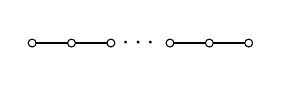
\begin{tikzpicture}[scale = 0.5]
\draw (0, 0) circle (0.1);
\draw (1, 0) circle (0.1);
\draw (2, 0) circle (0.1);
\node at (2.75, 0) {$\cdots$};
\draw (3.5, 0) circle (0.1);
\draw (4.5, 0) circle (0.1);
\draw (5.5, 0) circle (0.1);
\draw (0.1, 0) -- (0.9, 0);
\draw (1.1, 0) -- (1.9, 0);
\draw (3.6, 0) -- (4.4, 0);
\draw (4.6, 0) -- (5.4, 0);
\end{tikzpicture}
\end{tabular} & \begin{tabular}{l} $A_n$ \end{tabular} & \begin{tabular}{l}$(n+1)!$\end{tabular} \\
\begin{tabular}{l}
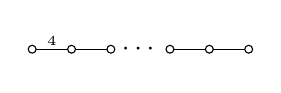
\begin{tikzpicture}[scale = 0.5]
\draw (0, 0) circle (0.1);
\draw (1, 0) circle (0.1);
\draw (2, 0) circle (0.1);
\node at (2.75, 0) {$\cdots$};
\draw (3.5, 0) circle (0.1);
\draw (4.5, 0) circle (0.1);
\draw (5.5, 0) circle (0.1);
\draw (0.1, 0) -- (0.9, 0);
\draw (1.1, 0) -- (1.9, 0);
\draw (3.6, 0) -- (4.4, 0);
\draw (4.6, 0) -- (5.4, 0);
\node at (0.5, 0.2) {\tiny{$4$}};
\end{tikzpicture}
\end{tabular}& \begin{tabular}{l}$B_n$\end{tabular} & \begin{tabular}{l}$2^n n!$\end{tabular} \\
\begin{tabular}{l}
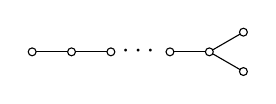
\begin{tikzpicture}[scale = 0.5]
\draw (0, 0) circle (0.1);
\draw (1, 0) circle (0.1);
\draw (2, 0) circle (0.1);
\node at (2.75, 0) {$\cdots$};
\draw (3.5, 0) circle (0.1);
\draw (4.5, 0) circle (0.1);
\draw ($(4.5, 0) + (30:1)$) circle (0.1);
\draw ($(4.5, 0) + (-30:1)$) circle (0.1);
\draw (0.1, 0) -- (0.9, 0);
\draw (1.1, 0) -- (1.9, 0);
\draw (3.6, 0) -- (4.4, 0);
\draw ($(4.5, 0) + (30:0.1)$) -- ($(4.5, 0) + (30:0.9)$);
\draw ($(4.5, 0) + (-30:0.1)$) -- ($(4.5, 0) + (-30:0.9)$);
\end{tikzpicture}
\end{tabular}& \begin{tabular}{l}$D_n$\end{tabular} & \begin{tabular}{l}$2^{n-1} n!$\end{tabular} \\
\begin{tabular}{l}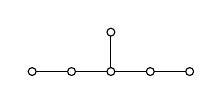
\begin{tikzpicture}[scale = 0.5]
\draw (0, 0) circle (0.1);
\draw (1, 0) circle (0.1);
\draw (2, 0) circle (0.1);
\draw (3, 0) circle (0.1);
\draw (4, 0) circle (0.1);
\draw (2, 1) circle (0.1);
\draw (0.1, 0) -- (0.9, 0);
\draw (1.1, 0) -- (1.9, 0);
\draw (2.1, 0) -- (2.9, 0);
\draw (3.1, 0) -- (3.9, 0);
\draw (2, 0.1) -- (2, 0.9);
\end{tikzpicture}\end{tabular}& \begin{tabular}{l}$E_6$\end{tabular} & \begin{tabular}{l}$72 \cdot 6!$\end{tabular} \\
\begin{tabular}{l}
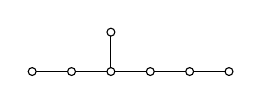
\begin{tikzpicture}[scale = 0.5]
\draw (0, 0) circle (0.1);
\draw (1, 0) circle (0.1);
\draw (2, 0) circle (0.1);
\draw (3, 0) circle (0.1);
\draw (4, 0) circle (0.1);
\draw (5, 0) circle (0.1);
\draw (2, 1) circle (0.1);
\draw (0.1, 0) -- (0.9, 0);
\draw (1.1, 0) -- (1.9, 0);
\draw (2.1, 0) -- (2.9, 0);
\draw (3.1, 0) -- (3.9, 0);
\draw (2, 0.1) -- (2, 0.9);
\draw (4.1, 0) -- (4.9, 0);
\end{tikzpicture}
\end{tabular}& \begin{tabular}{l}$E_7$\end{tabular} & \begin{tabular}{l}$72 \cdot 8!$\end{tabular} \\
\begin{tabular}{l}
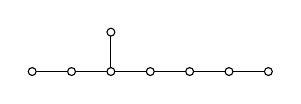
\begin{tikzpicture}[scale = 0.5]
\draw (0, 0) circle (0.1);
\draw (1, 0) circle (0.1);
\draw (2, 0) circle (0.1);
\draw (3, 0) circle (0.1);
\draw (4, 0) circle (0.1);
\draw (5, 0) circle (0.1);
\draw (6, 0) circle (0.1);
\draw (2, 1) circle (0.1);
\draw (0.1, 0) -- (0.9, 0);
\draw (1.1, 0) -- (1.9, 0);
\draw (2.1, 0) -- (2.9, 0);
\draw (3.1, 0) -- (3.9, 0);
\draw (2, 0.1) -- (2, 0.9);
\draw (4.1, 0) -- (4.9, 0);
\draw (5.1, 0) -- (5.9, 0);
\end{tikzpicture}
\end{tabular}& \begin{tabular}{l}$E_8$\end{tabular} & \begin{tabular}{l}$192 \cdot 10!$\end{tabular} \\
\begin{tabular}{l}
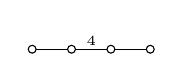
\begin{tikzpicture}[scale = 0.5]
\draw (0, 0) circle (0.1);
\draw (1, 0) circle (0.1);
\draw (2, 0) circle (0.1);
\draw (3, 0) circle (0.1);
\draw (0.1, 0) -- (0.9, 0);
\draw (1.1, 0) -- (1.9, 0);
\draw (2.1, 0) -- (2.9, 0);
\node at (1.5, 0.2) {\tiny{$4$}};
\end{tikzpicture}
\end{tabular}& \begin{tabular}{l}$F_4$\end{tabular} & \begin{tabular}{l}$1152$\end{tabular} \\
\begin{tabular}{l}
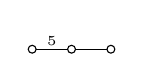
\begin{tikzpicture}[scale = 0.5]
\draw (0, 0) circle (0.1);
\draw (1, 0) circle (0.1);
\draw (2, 0) circle (0.1);
\draw (0.1, 0) -- (0.9, 0);
\draw (1.1, 0) -- (1.9, 0);
\node at (0.5, 0.2) {\tiny{$5$}};
\end{tikzpicture}
\end{tabular}& \begin{tabular}{l}$H_3$\end{tabular} & \begin{tabular}{l}$120$\end{tabular} \\
\begin{tabular}{l}
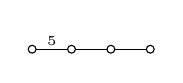
\begin{tikzpicture}[scale = 0.5]
\draw (0, 0) circle (0.1);
\draw (1, 0) circle (0.1);
\draw (2, 0) circle (0.1);
\draw (3, 0) circle (0.1);
\draw (0.1, 0) -- (0.9, 0);
\draw (1.1, 0) -- (1.9, 0);
\draw (2.1, 0) -- (2.9, 0);
\node at (0.5, 0.2) {\tiny{$5$}};
\end{tikzpicture}
\end{tabular}& \begin{tabular}{l}$H_4$\end{tabular} & \begin{tabular}{l}$14400$\end{tabular} \\
\begin{tabular}{l}
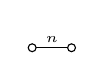
\begin{tikzpicture}[scale = 0.5]
\draw (0, 0) circle (0.1);
\draw (1, 0) circle (0.1);
\draw (0.1, 0) -- (0.9, 0);
\node at (0.5, 0.2) {\tiny{$n$}};
\end{tikzpicture}
\end{tabular}& \begin{tabular}{l}$I_2(n)$\end{tabular} & \begin{tabular}{l}$2n$\end{tabular}
\end{tabular}
\caption{Classification of Irreducible Finite Coxeter Groups}
\label{tab:classification}
\end{table}

\newpage


\section{Knot Theory}\label{sec:knot-theory}
\subsection{Knots and Links}
A \textit{knot} $K$ is the image of a smooth embedding of $S^1$ into $S^3$. A \textit{link} $L$ is a disjoint union of finitely many knots. Two links $L \subset S^3$ and $L' \subset S^3$ are said to be \textit{equivalent} if there exists an orientation-preserving diffeomorphism between the pair $(S^3, L)$ and the pair $(S^3, L')$, i.e., a diffeomorphism $S^3 \rightarrow S^3$ that restricts to a diffeomorphism of the links $L \rightarrow L'$.



\begin{example}[Torus Links]
Let $p, q$ be integers. Consider the universal covering $\mathbb{R}^2 \rightarrow T^2$, where the set $T^2 \subset \mathbb{R}^3$ is a standardly embedded torus. For an explicit parametrisation, consider e.g. Example~6 of Section 2-2 in Do Carmo's book \cite{docarmo1976}. Then the $(p,q)$-\textit{torus link} is the image of the lines through the points $\mathbb{Z}e_1$ of slope $p/q$.
\end{example}

\begin{example}[Pretzel Links]
The $(l_1, \dots, l_k)$-\textit{Pretzel link} is the link obtained by connecting twist regions in the way indicated in Figure \ref{fig:pretzel-link}. We will write $P(l_1, \dots, l_k)$ for this knot. An example is~drawn in Figure \ref{fig:p(2,3,-3)}.

\begin{figure}[ht]
\centering
\begin{minipage}{0.5\textwidth}
\centering
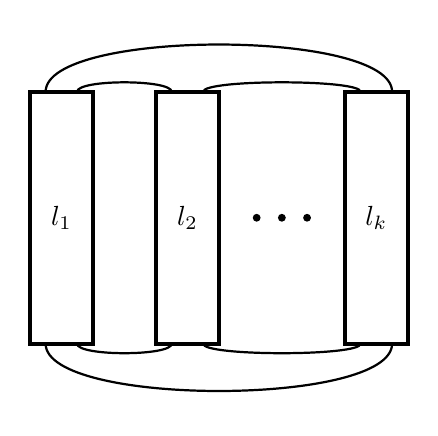
\begin{tikzpicture}[scale = 0.8]
\draw[ultra thick] (0, 0) rectangle (1,4);
\draw[ultra thick] (2, 0) rectangle (3, 4);
\node at (3.6, 2) [circle, fill, inner sep=1pt] {};
\node at (4,2) [circle, fill, inner sep=1pt] {};
\node at (4.4, 2) [circle, fill, inner sep=1pt] {};
\draw[ultra thick] (5, 0) rectangle (6, 4);

\begin{knot}
\strand[thick] (0.25, 4) .. controls +(0, 1) and +(0, 1) .. (5.75, 4);
\strand[thick] (0.75, 4) .. controls +(0, 0.2) and +(0, 0.2) .. (2.25, 4);
\strand[thick] (2.75, 4) .. controls +(0, 0.2) and +(0, 0.2) .. (5.25, 4);

\strand[thick] (0.25, 0) .. controls +(0, -1) and +(0, -1) .. (5.75, 0);
\strand[thick] (0.75, 0) .. controls +(0, -0.2) and +(0, -0.2) .. (2.25, 0);
\strand[thick] (2.75, 0) .. controls +(0, -0.2) and +(0, -0.2) .. (5.25, 0);
\end{knot}

\node at (0.5, 2) {$l_1$};
\node at (2.5, 2) {$l_2$};
\node at (5.5, 2) {$l_k$};

\end{tikzpicture}
\caption{$P(l_1, l_2, \dots, l_k)$}
\label{fig:pretzel-link}
\end{minipage}%
\begin{minipage}{0.5\textwidth}
\centering
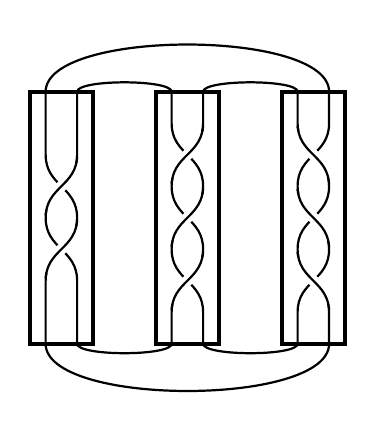
\begin{tikzpicture}[scale = 0.8]

\draw[ultra thick] (0, -0.5) rectangle (1, 3.5);
\draw[ultra thick] (2, -0.5) rectangle (3, 3.5);
\draw[ultra thick] (4, -0.5) rectangle (5, 3.5);

\begin{knot}[clip width = 5, flip crossing/.list={2, 4, 6, 8}]
\strand[thick] (0.25, -0.5) -- (0.25, 0.5) .. controls +(0, 0.5) and +(0, -0.5) .. (0.75, 1.5) .. controls +(0, 0.5) and +(0, -0.5) .. (0.25, 2.5) -- (0.25, 3.5);

\strand[thick] (0.75, -0.5) -- (0.75, 0.5) .. controls +(0, 0.5) and +(0, -0.5) .. (0.25, 1.5) .. controls +(0, 0.5) and +(0, -0.5) .. (0.75, 2.5) -- (0.75, 3.5);


\strand[thick] (2.25, -0.5) -- (2.25, 0) .. controls +(0, 0.5) and +(0, -0.5) .. (2.75, 1) .. controls +(0, 0.5) and +(0, -0.5) .. (2.25, 2) .. controls +(0, 0.5) and +(0, -0.5) .. (2.75, 3) -- (2.75, 3.5);

\strand[thick] (2.75, -0.5) -- (2.75, 0) .. controls +(0, 0.5) and +(0, -0.5) .. (2.25, 1) .. controls +(0, 0.5) and +(0, -0.5) .. (2.75, 2) .. controls +(0, 0.5) and +(0, -0.5) .. (2.25, 3) -- (2.25, 3.5);



\strand[thick] (4.25, -0.5) -- (4.25, 0) .. controls +(0, 0.5) and +(0, -0.5) .. (4.75, 1) .. controls +(0, 0.5) and +(0, -0.5) .. (4.25, 2) .. controls +(0, 0.5) and +(0, -0.5) .. (4.75, 3) -- (4.75, 3.5);

\strand[thick] (4.75, -0.5) -- (4.75, 0) .. controls +(0, 0.5) and +(0, -0.5) .. (4.25, 1) .. controls +(0, 0.5) and +(0, -0.5) .. (4.75, 2) .. controls +(0, 0.5) and +(0, -0.5) .. (4.25, 3) -- (4.25, 3.5);

\strand[thick] (0.75, -0.5) .. controls +(0, -0.2) and +(0, -0.2) .. (2.25, -0.5);
\strand[thick] (2.75, -0.5) .. controls +(0, -0.2) and +(0, -0.2) .. (4.25, -0.5);
\strand[thick] (0.25, -0.5) .. controls +(0, -1) and +(0, -1) .. (4.75, -0.5);


\strand[thick] (0.75, 3.5) .. controls +(0, 0.2) and +(0, 0.2) .. (2.25, 3.5);
\strand[thick] (2.75, 3.5) .. controls +(0, 0.2) and +(0, 0.2) .. (4.25, 3.5);
\strand[thick] (0.25, 3.5) .. controls +(0, 1) and +(0, 1) .. (4.75, 3.5);


\end{knot}
\end{tikzpicture}
\caption{$P(2, 3, -3)$}
\label{fig:p(2,3,-3)}
\end{minipage}
\end{figure}
\end{example}
\subsection{The Bridge Index}
Let $L \subset S^3$ be a link. The minimal number of local maxima of a smooth function $S^3 \rightarrow \mathbb{R}$ restricted to links isotopic to $L$ is called the \textit{bridge index} of $L$ and referred to as $b(L)$.
This can be diagrammatically characterized in the following way. Let $D$ be a diagram of $L$. An \textit{arc} in $D$ is a segment of $D$ beginning and ending with an undercrossing, containing no undercrossings in between. A \textit{bridge} of $D$ is an arc of $D$ that contains at least one overcrossing.

\begin{proposition}
The bridge index of a link $L \subset S^3$ is equal to the number of bridges in a diagram~$D$ of $L$, minimized over all diagrams.
\end{proposition}

\begin{proof}[Proof idea]
It suffices to run over embeddings in $\mathbb{R}^3$ and only consider the function mapping a point in $\mathbb{R}^3$ to its $z$-coordinate.
Note that a bridge of a diagram induces a maximum of the height function when flipping the diagram to its side and vice versa.
\end{proof}

%TODO prove or cite


The following was first proven by Schubert \cite{schubert1954}.

\begin{proposition}\label{prop:bridge-index-connected-sum}
Let $K$ and $K'$ be knots. Then $b(K\#K') = b( K ) + b(K') - 1$.
\end{proposition}


\subsection{The Link Group}\label{subsec:link-group}
The \textit{link group} $\pi(L)$ of a link $L \subset S^3$ is the fundamental group of its complement in $S^3$. In symbols this reads $\pi(L) = \pi_1(S^3 \setminus L)$. If $L$ is a knot $K$ then the link group $\pi(K)$ is referred to as its \textit{knot group}.

The knot group essentially classifies all knots, in that if two prime knots have isomorphic knot groups then they are either equivalent or mirrors of each other \cite{gordon1989}. Be warned that this is no longer true for links, see \cite{rolfsen2003}. This suggests that studying the knot group might be just as good as studying knots themselves.

We will now describe an algorithm that computes the link group of an oriented link. Let $L \subset S^3$ be a link and let $D$ be any diagram of $L$. Let $S = \{m_1, \dots, m_k\}$ be the set of diagram meridians, oriented from right to left. A meridian $m_i$ should be interpreted at as the meridian starting at the reader's eye, which will serve as the base point of the fundamental group, passing under the arc and going back to the reader's eye without any detour.
Having assigned a generator to every crossing, we now assign a relator $r$ to any crossing, as indicated in Figure \ref{fig:wirtinger-relations}.

\begin{figure}[ht]
\centering
\begin{minipage}{.5\textwidth}
\centering
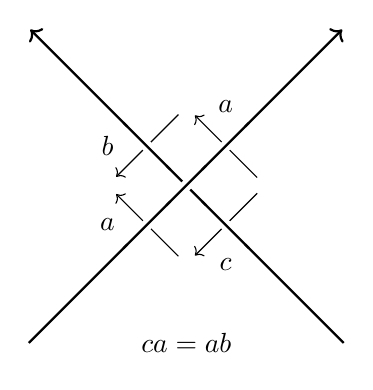
\begin{tikzpicture}
\begin{knot}[clip width = 5]
\strand[black, thick, ->] (0, 0) -- (4, 4);
\strand[black, thick, ->] (4, 0) -- (0, 4);

\strand[black, ->] (1.9, 1.1) -- (1.1, 1.9);
\strand[black, ->] (1.9, 2.9) -- (1.1, 2.1);
\strand[black, ->] (2.9, 2.1) -- (2.1, 2.9);
\strand[black, ->] (2.9, 1.9) -- (2.1, 1.1);

\node at (1, 1.5) {$a$};
\node at (1, 2.5) {$b$};
\node at (2.5, 3) {$a$};
\node at (2.5, 1) {$c$};

\node at (2, 0) {$ca = ab$};
\end{knot}
\end{tikzpicture}
\end{minipage}%
\begin{minipage}{.5\textwidth}
\centering
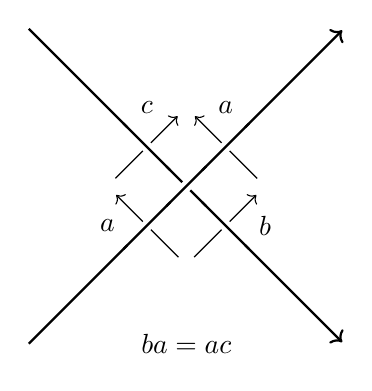
\begin{tikzpicture}
\begin{knot}[clip width = 5]
\strand[black, thick, ->] (0, 0) -- (4, 4);
\strand[black, thick, ->] (0, 4) -- (4, 0);

\strand[black, ->] (1.9, 1.1) -- (1.1, 1.9);
\strand[black, ->] (1.1, 2.1) -- (1.9, 2.9);
\strand[black, ->] (2.9, 2.1) -- (2.1, 2.9);
\strand[black, ->] (2.1, 1.1) -- (2.9, 1.9);

\node at (1, 1.5) {$a$};
\node at (1.5, 3) {$c$};
\node at (2.5, 3) {$a$};
\node at (3, 1.5) {$b$};

\node at (2, 0) {$ba = ac$};
\end{knot}
\end{tikzpicture}
\end{minipage}
\caption{Relations in the Wirtinger Presentation}
\label{fig:wirtinger-relations}
\end{figure}

Since it is very well known that this procedure works, it would be reasonable to omit the proof. But we are going to steal the argument and apply it to slice disks later on (see Section \ref{subsec:ribbons}), so it will be useful to go over the proof again quickly.



\begin{figure}[htb]
\centering
\begin{tikzpicture}
\begin{knot}[clip width = 5, ignore endpoint intersections = false]
\strand[thick] (-2.5, 2.5) -- (-2.5, 3.5);

\strand[thick] (-2.333, -1) -- (-0.667, 4);
\strand[thick] (2, 2.5) --(-0, 2.5) .. controls +(-0.25, 0) and +(0.25, 0) .. (-0.5, 1.5);
\strand[thick] (-2.5, 1.5) .. controls +(-0.25, 0) and +(0.25, 0) .. (-3, 2.5) -- (-4.5, 2.5);
\strand[thick] (0, 0) -- (-4, 0) -- (-3, 3) -- (1, 3) -- (0, 0);
%\strand[thick] (0, 0) -- (0, -1.5);
%\strand[thick] (-4, 0) -- (-4, -1.5);
%\strand[thick] (1, 3) -- (1, 1.5);
\strand[->] (-1.5, 2) .. controls +(-0.167, 0) and +(0, 0.5) .. (-3, 1.5);
\strand (-3, 1.5) .. controls +(0, -0.5) and +(-0.167, 0) .. (-1.5, 1)
	.. controls +(0.167, 0) and +(0, -0.5) .. (0, 1.5)
	.. controls +(0, 0.5) and +(0.167, 0) .. (-1.5, 2);
%\strand (-1.5, 1.5) ellipse (1.5 and 0.5);

\strand[->] (-4, 2) -- (-3.667, 3);
\strand[->] (1.333, 2) -- (1.667, 3);
\strand[->] (-2.667, -0.5) -- (-1.667, -0.5);
\strand[->] (-1.33, 3.5) -- (-0.333, 3.5);
\end{knot}


\fill[opacity=0.2] (0, 0) -- (-4, 0) -- (-3, 3) -- (1, 3) -- (0, 0);
%\fill[opacity=0.2] (1, 3) -- (0, 0) -- (0, -1.5) -- (1, 1.5) -- (1, 3);
%\fill[opacity=0.2] (0, 0) -- (0, -1.5) -- (-4, -1.5) -- (-4, 0);
\draw[dashed] (-0.5, 1.5) -- (-2.5, 1.5); 

\node at (-2.5, 3.5) [circle, fill, inner sep=1pt]{};
\node at (-2.5, 3.7) {$x$};
\node at (-3.67, 3.2) {$b$};
\node at (1.7, 3.2) {$c$};
\node at (-1.467, -0.5) {$a$};
\node at (-0.133, 3.5) {$a$};
\node at (-3.2, 1.3) {$\gamma$};

\end{tikzpicture}
\caption{Explanation of the Wirtinger relations}
\label{fig:proof-of-wirtinger}
\end{figure}



\begin{theorem}\label{thm:wirtinger-thm}
Let $L$ be a link.
Then the presentation resulting from performing the Wirtinger algorithm is a presentation of the link group $\pi(L)$.
\end{theorem}


\begin{proof}
This is the proof given in \cite{rolfsen2003}. In order to apply van Kampen's theorem \cite{hatcher2002}, first we make sure that $L$ lies entirely in the plane $P$, except for the crossings, where the understrand passes under the plane. Suppose all understrands reach the same maximal distance~$\varepsilon$ to $P$ and reach it in exactly one connected component of $K$ intersected with $P^{-}$. Here $P^-$ is the plane parallel to $P$ of distance~$\varepsilon$ in the down-direction, marked in grey in Figure \ref{fig:proof-of-wirtinger}.
Position the base point $x$ somewhere above $P$. We now subdivide $S^3$ as follows.
Let $H^+$ be the closed half-space above $P^-$ intersected with the link complement. Then $H^+$ contains $x$. Moreover, the fundamental group of $H^+$ is free with generating set the meridians of $L$. Similarly, let $H^-$ be the closed half-space below $P^-$, also intersected with $K$. In contrast to $H^+$ we have that $H^-$ is simply connected.

The fundamental group of $P^-$ is also free, but the generators this time are curves like $\gamma$ in Figure~\ref{fig:proof-of-wirtinger}. In $H^-$, these curves are trivial because $H^-$ is simply connected. On the other hand, in $H^+$ they represent words like $b^{-1}aca^{-1}$, where $a, b$ and $c$ are diagram meridians (or inverses thereof) of arcs close to the crossing considered. These are exactly the Wirtinger relations.
By van Kampen's Theorem, these relations yield a presentation of the link complement, which is what we wanted to show.
\end{proof}

\begin{theorem}\label{thm:mr<=b}
Let $L \subset S^3$ be a link. Then $\mu(L) \leq b(L)$.
\end{theorem}

\begin{proof}
This is very similar to the proof of Theorem \ref{thm:wirtinger-thm}. This time we don't dip down for undercrossings as in Figure \ref{fig:proof-of-wirtinger} but we stay up as long as possible after the overcrossings. Then the generators given by the van Kampen argument are precisely the bridges in the diagrammatic interpretation of bridges.
\end{proof}

\newpage


\section{Coxeter Quotients}
\subsection{The Reflection Quotient}\label{subsec:reflection-quotient}
Let $L \subset S^3$ be a link. A \textit{Coxeter quotient} is a quotient $\pi(K)/N$ of the link group which is isomorphic to a Coxeter group $W$ such that every meridian in $\pi(L)$ corresponds to a reflection in $W$.
In many cases, finding Coxeter quotients of links is rather straight-forward, at least with the help of a computer. This is because checking whether a specific set of Coxeter relations induces a Coxeter quotient of a link amounts to checking the validity of the defining relations of its link group.

The \textit{reflection quotient} is the group $r(L) = \pi_1(S^3 \setminus L) / \langle \langle m^2 \rangle \rangle$, where $m$ is any meridian of $L$. Because it is clumsy to write down a presentation in this fashion we agree to add the relations $s^2$ for all generators $s$ in $S$ when writing a presentation as $\langle S \; | \; R \rangle^{(2)}$. Using this notation, the reflection quotient can be defined to be
$$r(L) = \pi(L)^{(2)}.$$

Coxeter quotients of a link $L$ are also quotients of $r(L)$. The fact justifying the study of quotients of $r(K)$ lies in the following theorem.

\begin{theorem}[Boileau-Zimmermann \cite{boileau1989}, Theorem 1]
Let $K$ and $K'$ be prime knots such that $r(K)$ and $r(K')$ are infinite. Then $K$ and $K'$ are equivalent if and only if $r(K)$ and $r(K')$ are isomorphic.
\end{theorem}

%Be warned that in \cite{boileau1989} the reflection quotient is denoted $O(L)$ and is called the $\pi$-orbifold group.

It is easy to write down a presentation of the reflection quotient from a presentation of the link group $\pi(L) = \langle S \; | \; R \rangle$ of a link $L \subset S^3$. Just add the relations $s^2$ for all $s$ in $S$, and simplify $R$ by replacing all occurrences of $s^{-1}$ by $s$ and all occurrences of $s^2$ by the empty word. These presentations are generally shorter, easier to read and less prone to mistakes since it is no longer possible to confuse meridians with their inverses.
Note in addition that the Wirtinger algorithm (see Section \ref{subsec:link-group}) can be simplified so that the relation $ca = ab$ in Figure \ref{fig:wirtinger-relations} reads $acab = 1$ in the reflection quotient.
We will now mainly consider the reflection quotient instead of the link group.


\begin{figure}[ht]
\centering
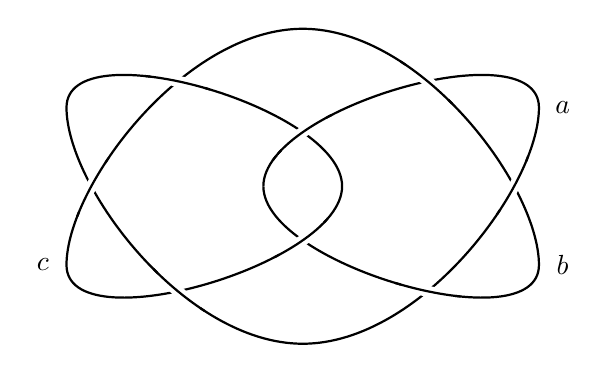
\begin{tikzpicture}
\begin{knot}[consider self intersections = true, clip width = 5, ignore endpoint intersections=false,
%draft mode = crossings,
flip crossing/.list={3, 5, 7}]
\strand[thick] (-0.5, 0) .. controls +(0, 1) and +(0, 1) .. (3, 1) .. controls +(0, -1) and +(1.5, 0) .. (0, -2) .. controls +(-1.5, 0) and +(0, -1) .. (-3, 1) .. controls +(0, 1) and +(0, 1) .. (0.5, 0) .. controls +(0, -1) and +(0, -1) .. (-3, -1) .. controls +(0, 1) and +(-1.5, 0) .. (0, 2) .. controls +(1.5, 0) and +(0, 1) .. (3, -1) .. controls +(0, -1) and +(0, -1) .. (-0.5, 0);
\end{knot}

\node at (3.3, 1) {$a$};
\node at (3.3, -1) {$b$};
\node at (-3.3, -1) {$c$};
\end{tikzpicture}
\caption{The knot $8_5$}
\label{fig:8-5}
\end{figure}

\begin{example}[The Knot $8_5$]
Consider $K = 8_5$ from Rolfsen's knot table, compare Figure \ref{fig:8-5}. Then~$K$ has a Coxeter quotient with graph $A_3 =\coxtwothreethree$, whose associated Coxeter group is isomorphic to the permutation group $S_4$.
Note that by the Wirtinger algorithm, the reflection quotient (defined in Section \ref{subsec:reflection-quotient}) has a presentation
$$r(8_5) = \langle a, b, c\; | \; babc(ba)^2bc(ba)^4, babc(ba)^4cbabc(ab)^2a \rangle^{(2)}.$$
%TODO check this
These relations are satisfied in the Coxeter group
$$W = \langle a, b, c \; | \; (ab)^2, (ac)^3, (bc)^3 \rangle^{(2)}.$$
Thus, $W$ is a quotient of $\pi_1(S^3 \setminus 8_5)$.
\end{example}

Note that there exist presentations of the knot group of $8_5$, for example, any presentation involving more than three meridians, such that the above method does not work. It is thus difficult to prove in general that a fixed link $L$ does not admit a Coxeter quotient isomorphic to a specific Coxeter group~$W$.

\subsection{List of Coxeter Knots}\label{subsec:list-of-quotients}
The following list of Coxeter knots in Rolfsen's table \cite{rolfsen2003} was found using the following algorithm. First, compute a presentation of the reflection quotient using the Wirtinger algorithm, modified such that the presentation does not use more generators than the bridge index of the knot in question. Then, use some solution of the word problem in Coxeter groups to find all Coxeter quotients that map generating meridians to generating reflections. Note that this algorithm may not detect all Coxeter knots.

Because all $2$-bridge knots are Coxeter (see Section \ref{subsec:rank-two}), Table \ref{tab:cox-quotients} consists of all $3$-bridge knots in Rolfsen's table with up to nine crossings that were found to be Coxeter by the above algorithm.

\begin{table}[htb]
\centering
\begin{minipage}[t]{0.45\textwidth}
\centering
\begin{tabular}[t]{c|c}
Knot & Coxeter Quotients \\
\hline
$8_5$ & \coxtwothreethree \\
$8_{10}$ & \coxtwothreethree \\
$8_{15}$ & \coxtwothreethree \\
$8_{19}$ & \coxtwothreethree \\
$8_{20}$ & \coxtwothreethree \\
$8_{21}$ & \coxtwothreethree \\
$9_{16}$ & \coxtwothreethree \\
$9_{22}$ & \coxathreetype{$5$} \\
$9_{24}$ & \coxtwothreethree \\
$9_{25}$ & \coxathreetype{$5$} \\
$9_{28}$ & \coxtwothreethree \\
$9_{30}$ & \coxathreetype{$5$} \\
\end{tabular}
\end{minipage}%
\begin{minipage}[t]{0.55\textwidth}
\centering
\begin{tabular}[t]{c|c}
Knot & Coxeter Quotients \\
\hline
\verticalcenter{$9_{35}$}\rule{0pt}{4ex} & \verticalcenter{\verticalcenter{\coxtwothreethree} and \verticalcenter{\coxthreethreethree}} \\
\verticalcenter{$9_{36}$} & \coxathreetype{$5$} \\
\verticalcenter{$9_{37}$} &
\verticalcenter{\verticalcenter{\coxtwothreethree} and
\verticalcenter{\coxthreethreethree}} \\
\verticalcenter{$9_{40}$} & $\;\;\,$\verticalcenter{\coxtwothreethree} and \verticalcenter{\coxathreetype{$5$}} \\
\verticalcenter{$9_{42}$} & \coxathreetype{$5$} \\
\verticalcenter{$9_{43}$} & \coxathreetype{$5$} \\
\verticalcenter{$9_{44}$} & \coxathreetype{$5$} \\
\verticalcenter{$9_{45}$} & \coxathreetype{$5$} \\
\verticalcenter{$9_{46}$} &
\verticalcenter{\verticalcenter{\coxtwothreethree} and
\verticalcenter{\coxthreethreethree}} \\
\verticalcenter{$9_{48}$} &
\verticalcenter{\verticalcenter{\coxtwothreethree} and
\verticalcenter{\coxthreethreethree}} \\
\end{tabular}
\end{minipage}
\caption{List of Coxeter knots with bridge index $3$}
\label{tab:cox-quotients}
\end{table}

The $3$-bridge knots that were not found to have a rank $3$ Coxeter quotient are $8_{16}, 8_{17}$, $8_{18}$, $9_{29}$, $9_{32}$, $9_{33}$, $9_{34}$, $9_{38}, 9_{39}, 9_{41}, 9_{47}$ and $9_{49}$. Note that it remains open whether any of those knots admit a Coxeter quotient of rank $3$.
Data concerning knots of crossing number $10$ can be found in Appendix~\ref{sec:data}.

\subsection{Meridional Rank}\label{subsec:meridional-rank}
For a link $L$ we define its \textit{meridional rank} to be the least possible number of meridians of $L$ needed to generate the group $\pi(L)$. Here, a \textit{meridian} is any generator of $H_1(S^3 \setminus L) = \pi(L)^{\text{ab}}$.
We define the \textit{Coxeter rank} of a link $L$, abbreviated $c (L)$, to be the maximal number $n$ such that $L$ has a Coxeter quotient of rank $n$. Abbreviating the bridge index of $L$ by $b(L)$, we have the following.

\begin{theorem}\label{thm:c<=mu<=b}
Let $L \subset S^3$ be any link. Then we have $c(L) \leq \mu(L) \leq b(L)$.
\end{theorem}

\begin{proof}
The inequality $\mu( L ) \leq b(L)$ is Theorem \ref{thm:mr<=b}. Moreover, $c (L) \leq \mu( L )$, is a direct consequence of the fact that the number of generating reflections is determined by the Coxeter system. For a proof, see for example Lemma 2.1 in \cite{felikson2009}.
\end{proof}

Let us refer to a link $L \subset S^3$ that has a Coxeter quotient of rank $n = b(L)$ as a \textit{Coxeter link}. Then we obtain the following from $c(L) \geq b(L)$ together with Theorem \ref{thm:c<=mu<=b}.

\begin{corollary}\label{cor:coxeter-links-meridional-rank}
Coxeter links satisfy the meridional rank conjecture.
\end{corollary}

Another application of the techniques we have developed so far lies in the following.

\begin{theorem}\label{thm:connected-sums-coxeter-rank}
Let $K$ and $K'$ be knots. Then $c (K\#K') = c (K) + c (K') - 1$.
\end{theorem}

\begin{proof}
Let $W$ and $W'$ be Coxeter quotients of $K$ and $K'$, respectively. First we choose diagrams of $K$ and $K'$ such that the generators of $\pi(K)$ and $\pi(K')$ that get mapped to generating reflections of $W$ and $W'$ are diagram meridians. Let $s \in \pi(K)$ and $s' \in \pi(K')$ each be one of those diagram meridians.

Now observe that $\pi(K\#K')$ is of the form $\pi(K) * \pi(K') / ss'$. Thus, we can explicitly write down a Coxeter quotient of $K\#K'$ as follows. Let $\Gamma$ and $\Gamma'$ be the Coxeter graphs associated to $W$ and $W'$. Then there is a Coxeter quotient of $K\#K'$ with graph
\begin{center}
\begin{tikzpicture}
\draw[dashed] (0.85, 0.15) -- (0.15, 0.85);
\draw[dashed] (-0.15, 0.85) -- (-0.85, 0.15);
\draw (0.8, 0) -- (-0.8, 0);

\node at (0, 1) {$s$};
\node at (-1, 0) {$\Gamma$};
\node at (1, 0) {$\Gamma'$};
\node at (0, 0.2) {$\infty$};
\end{tikzpicture}
\end{center}
which has rank $\text{rk } W + \text{rk } W' - 1$. This proves that $c(K\#K') \geq c(K) + c(K') -1$. The other inequality follows from the fact that any maximal Coxeter quotient of $K\#K'$ induces Coxeter quotients of $K$ and of $K'$ whose ranks add up to $c(K\#K') + 1$.
\end{proof}

\begin{corollary}
There are knots of arbitrarily high meridional rank.
\end{corollary}

\begin{proof}
Just take connected sums of your favorite two-bridge knot.
\end{proof}

\begin{corollary}
Connected sums of Coxeter knots are Coxeter knots.
\end{corollary}

\begin{proof}
Let $J, K \subset S^3$ be arbitrary knots. Then we have already shown that $b(J\#K) = b(J) + b(K) - 1$ and $c (J\#K) \leq b(J\#K)$. If $J$ and $K$ are both Coxeter knots then equality immediately follows from Theorem \ref{thm:connected-sums-coxeter-rank}.
\end{proof}

\subsection{Rank Two Quotients}\label{subsec:rank-two}
In this section we have a particularly close look at dihedral quotients of link groups. As we shall see, this is closely related to a popular notion in the literature, described for example in \cite{przytycki1998}. 

Let $L$ be a link. We will refer to a homomorphism $c: \pi(L) \rightarrow D_n$ mapping all meridians of $L$ to reflections in $D_n$ as a \textit{Fox $n$-coloring}. Note that a surjective Fox $n$-coloring is a dihedral quotient of $L$. We will call a Fox $n$-coloring $c$ \textit{non-trivial} if the image of $c$ contains more than one reflection in $D_n$, and we will call a link $L$ \textit{Fox $n$-colorable} if $L$ admits a non-trivial Fox $n$-coloring. Note that any link admits trivial Fox $n$-colorings for all $n$.

\begin{example}[Fox $3$-colorings]
Let $a, b, c$ be the reflections of $D_3$. Then a Fox $3$-coloring of $L$ is just a labeling of the arcs in a diagram of $L$ such that at any crossing either only one symbol or all three symbols appear.

The reader may convince themselves of the fact that the trefoil knot in Figure \ref{fig:trefoil} is Fox $3$-colorable, whereas the figure-eight knot in Figure \ref{fig:figure-8} is not.

\begin{figure}[ht]
\centering
\begin{minipage}{0.5\textwidth}
 \centering
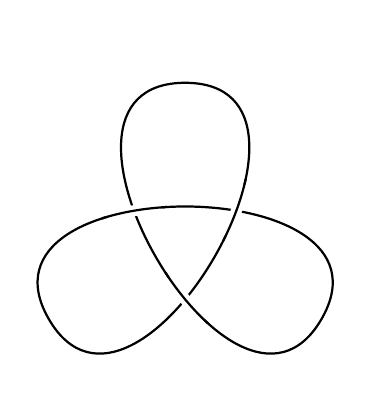
\begin{tikzpicture}
\clip (-2, -1.6) rectangle (2,2.7);
\begin{knot}[clip width = 5, consider self intersections = true, flip crossing = 2]

\strand[black, thick] (0,2) .. controls +(2.2,0) and +(120:-2.2) .. (210:2) .. controls +(120:2.2) and +(60:2.2) .. (-30:2) .. controls +(60:-2.2) and +(-2.2,0) .. (0,2);
\end{knot}
\end{tikzpicture}
\caption{The Trefoil Knot}
\label{fig:trefoil}
\end{minipage}%
\begin{minipage}{0.5\textwidth}
\centering
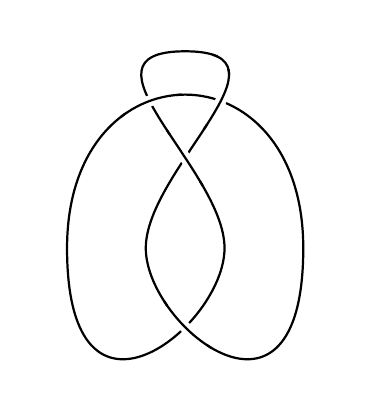
\begin{tikzpicture}
\clip (-2, -2.5) rectangle (2, 1.8);
\begin{knot}[consider self intersections = true, ignore endpoint intersections=false, clip width = 5, flip crossing = 2]
\strand[thick] (0, 1.5) .. controls +(1.5, 0) and +(0, 1) .. (-0.5, -1) .. controls +(0, -1) and +(0, -2.6) .. (1.5, -1) .. controls +(0, 2.6) and +(0, 2.6) .. (-1.5, -1) .. controls +(0, -2.6) and +(0, -1) .. (0.5, -1) .. controls +(0, 1) and +(-1.5, 0) .. (0, 1.5);
\end{knot}
\end{tikzpicture}
\caption{The Figure-Eight Knot}
\label{fig:figure-8}
\end{minipage}
\end{figure}
\end{example}

Let $n$ be a prime number. We will now present an algorithm to check whether a given link $L$ is $n$-colorable. First we make the following identification of the set of reflections with $\mathbb{Z}_n$. Write $$D_n = \langle a, b \; | \; (ab)^n \rangle^{(2)}.$$ Then the set $R$ of reflections is the set of elements of the form $(ab)^ka$. We will identify this reflection with the element $k$ in $\mathbb{Z}_p$.
Under this identification, the Wirtinger relation at any crossing reads $$2k = i + j,$$ see Figure \ref{fig:wirtinger-dihedral}. Indexing the set of diagram meridians and the set of crossings in some manner we can interpret this as a system of linear equations over $\mathbb{Z}$. Let us call the matrix of this system $\widehat{C}$. Note that this system admits trivial solutions, namely the ones assigning the same element of $\mathbb{Z}$ to all diagram meridians. Ignoring this set of solutions corresponds to deleting a row and a column of $\widehat{C}$ to obtain what we will call the \textit{coloring matrix} $C$.

\begin{figure}[ht]
\centering
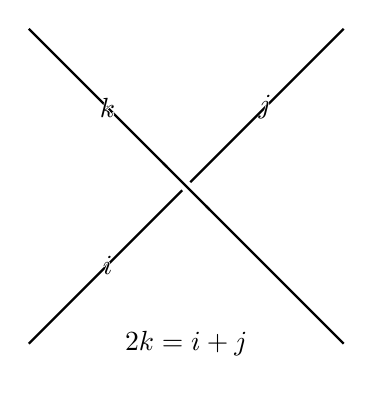
\begin{tikzpicture}
\begin{knot}[clip width = 5, flip crossing = 1]
\strand[thick] (-2, -2) -- (2, 2);
\strand[thick] (-2, 2) -- (2, -2);
\end{knot}
\node at (-1, -1) {\contour{white}{$i$}};
\node at (1, 1) {\contour{white}{$j$}};
\node at (-1, 1) {\contour{white}{$k$}};
\node at (0, -2) {$2k = i + j$};
\end{tikzpicture}
\caption{The Wirtinger relation at a crossing after identification of diagram meridians with $\mathbb{Z}_p$}
\label{fig:wirtinger-dihedral}
\end{figure}


\begin{lemma}
Let $L$ be any link and $n$ be prime. Then $L$ is Fox $n$-colorable if and only if $n$ divides $\det C$, where $C$ is the coloring matrix of $L$.
\end{lemma}

\begin{proof}
The condition for the linear system described above to have non-trivial solutions is for $C$ to be singular over $\mathbb{Z}_n$, which is obviously equivalent to $n$ dividing $\det C$ as a matrix with integer coefficients.
\end{proof}

One can prove that the determinant of $C$ neither depends on the diagram, nor on the choice of which row and column to delete from $\widehat{C}$. For this reason, we will refer to the determinant $\det C$ simply as the \textit{determinant} of $L$, written $\det L$. In the literature the determinant of $L$ is usually defined to be its Alexander polynomial evaluated at $-1$, but it turns out that these definitions are actually equivalent. %TODO cite nafies book

\begin{example}
Consider the Trefoil $K$ indexed as in Figure \ref{fig:trefoil-labeled-for-coloring}.
\begin{figure}[ht]
\centering
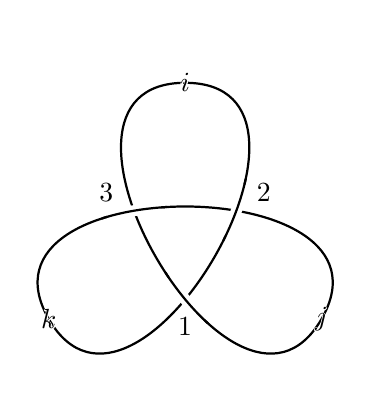
\begin{tikzpicture}
\clip (-2, -1.6) rectangle (2,2.7);
\begin{knot}[clip width = 5, consider self intersections = true, flip crossing = 2]

\strand[black, thick] (0,2) .. controls +(2.2,0) and +(120:-2.2) .. (210:2) .. controls +(120:2.2) and +(60:2.2) .. (-30:2) .. controls +(60:-2.2) and +(-2.2,0) .. (0,2);
\end{knot}
\node at (0, 2) {\contour{white}{$i$}};
\node at (210:2) {\contour{white}{$k$}};
\node at (-30:2) {\contour{white}{$j$}};

\node at (0, -1.1) {$1$};
\node at (-1, 0.6) {$3$};
\node at (1, 0.6) {$2$};
\end{tikzpicture}
\caption{The Trefoil Knot with labels}
\label{fig:trefoil-labeled-for-coloring}
\end{figure}

Then the linear equations read $2i = j + k$, $2j = i + k$ and $2k = i + j$, corresponding to the matrix
$$\widehat{C} = \left(\begin{matrix}
2 & -1 & -1 \\
-1 & 2 & -1 \\
-1 & -1 & 2
\end{matrix}\right).$$
Deleting from $\widehat{C}$ the last row and the last column we obtain the coloring matrix
$$C = \left( \begin{matrix}
2 & -1 \\
-1 & 2
\end{matrix} \right),$$
yielding that $\det K = 3$. Note that this agrees with the previous observation that $K$ is Fox $3$-colorable.
\end{example}

It can be shown that the determinant of a 2-bridge link $L$ is never equal to one. This implies that~$L$ has a dihedral quotient. Thus, all 2-bridge links are Coxeter.

%We are now ready to eliminate $2$-bridge knots from all our %discussions with the techniques developed here. The key to this %lies in the following.

%\begin{theorem}
%Let $K$ be a $2$-bridge link. Then $\det L > 1$.
%\end{theorem}
%TODO prove and cite

%\begin{corollary}
%All $2$-bridge links are Coxeter.
%\end{corollary}

\subsection{Realization}
%TODO describe this more clearly.
In this section we are going to show that many Coxeter groups are Coxeter quotients of knots. In fact, \textit{all} Coxeter groups are Coxeter quotients of links.

\begin{proposition}\label{prop:trivial-realization}
Let $L$ be the trivial link on $n$ components. Then the link group $\pi(L)$ is free on $n$ generators which are meridians. In particular, any Coxeter group $W$ is a Coxeter quotient of $\pi(L)$.
\end{proposition}

Since this is a little underwhelming we will try to do better. The following construction is essentially due to Brunner \cite{brunner1992}.

\begin{algo}[Brunner's Construction]\label{algo:brunner's-construction}
Let $\Gamma$ be any Coxeter graph, this time with edges labeled $2$ for commuting generators and no edge for no relations (contrary to the convention above). If $\Gamma$ is not planar, choose a maximal planar subgraph instead of $\Gamma$ and fix an embedding of $\Gamma$ into the plane.

Now consider the dual graph $\Gamma^*$ of $\Gamma$ whose vertices are the faces of $\Gamma$, with edges weighted $m$ connecting vertices $s, t$ if and only if there is an edge labeled $m$ separating the faces of $\Gamma$ corresponding to $s, t$. Note that $\Gamma^*$ is not necessarily a simple graph, even if $\Gamma$ is (e.g., if $\Gamma$ is a tree).

We now interpret $\Gamma^*$ as a set of instructions how to construct a surface $S$ whose boundary will be a link $L(\Gamma^*)$ admitting a Coxeter quotient isomorphic to the Coxeter group corresponding to $\Gamma$. First, blow up the vertices of $\Gamma^*$ to disks. Now replace each edge labelled $m$ between disks by bands with $m$ twists. This procedure is illustrated in Figure \ref{fig:brunners-construction}.
\end{algo}

\begin{figure}[htb]
\centering
\begin{minipage}{0.37\textwidth}
\centering
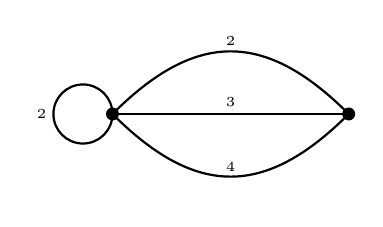
\begin{tikzpicture}[scale = 0.75]
\draw[thick] (0, 0) -- (4, 0);
\draw[thick] (0, 0) .. controls +(45:2) and +(315:-2) .. (4, 0);
\draw[thick] (0, 0) .. controls +(315:2) and +(45:-2) .. (4, 0);
\draw[thick] (-0.5, 0) circle (0.5);

\draw[fill = black] (0, 0) circle (0.1);
\draw[fill = black] (4, 0) circle (0.1);

\node at (2, 1.23) {\tiny{$2$}};
\node at (2, 0.2) {\tiny{$3$}};
\node at (2, -0.9) {\tiny{$4$}};
\node at (-1.2, 0) {\tiny{$2$}};
\end{tikzpicture}
\end{minipage}%
\begin{minipage}{0.63\textwidth}
\centering
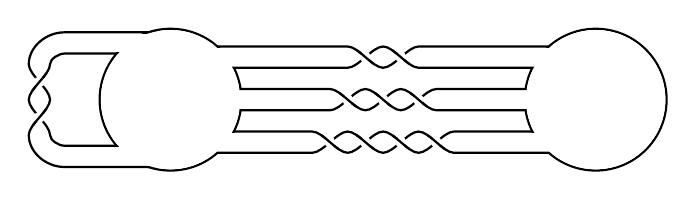
\begin{tikzpicture}[scale = 0.45]
\draw[thick] (0, 0) circle (2);
\draw[thick] (12, 0) circle (2);
\filldraw[color=white] (0, 0.95) -- (4, 0.95) -- (4, 1.45) --								  (0, 1.45);
\filldraw[color=white] (0, 0.25) -- (4, 0.25) -- (4, -0.25) --
							  (0, -0.25);
\filldraw[color=white] (0, -0.95) -- (4, -0.95) -- (4, -1.45)
							  -- (0, -1.45);
\filldraw[color=white] (0, 1.85) -- (-2, 1.85) -- (-2, 1.35)
								-- (0, 1.35);
\filldraw[color=white] (0, -1.85) -- (-2, -1.85) -- (-2, -1.35)
								-- (0, -1.35);
\filldraw[color=white] (12, 0.95) -- (8, 0.95) -- (8, 1.45) --								  (12, 1.45);
\filldraw[color=white] (12, 0.25) -- (8, 0.25) -- (8, -0.25) --
							  (12, -0.25);
\filldraw[color=white] (12, -0.95) -- (8, -0.95) -- (8, -1.45)
							  -- (12, -1.45);

\begin{knot}[clip width = 5, ignore endpoint intersections=false,
clip radius=2pt,
flip crossing/.list = {1, 4, 7, 9, 10}]

\strand[thick] (0, 0.9) -- (5, 0.9) .. controls +(0.3, 0) and +(-0.3, 0)
				 .. (6, 1.5) .. controls +(0.3, 0) and +(-0.3, 0)
				 .. (7, 0.9) -- (12, 0.9);
				 
\strand[thick] (0, 1.5) -- (5, 1.5) .. controls +(0.3, 0) and +(-0.3, 0)
				 .. (6, 0.9) .. controls +(0.3, 0) and +(-0.3, 0)
				 .. (7, 1.5) -- (12, 1.5);

\strand[thick] (0, 0.3) -- (4.5, 0.3) .. controls +(0.3, 0) and +(-0.3, 0)
			   .. (5.5, -0.3) .. controls +(0.3, 0) and +(-0.3, 0)
			   .. (6.5, 0.3) .. controls +(0.3, 0) and +(-0.3, 0)
			   .. (7.5, -0.3) -- (12, -0.3);
\strand[thick] (0, -0.3) -- (4.5, -0.3) .. controls +(0.3, 0) and +(-0.3, 0)
				.. (5.5, 0.3) .. controls +(0.3, 0) and +(-0.3, 0)
				.. (6.5, -0.3) .. controls +(0.3, 0) and +(-0.3, 0)
				.. (7.5, 0.3) -- (12, 0.3);
				
\strand[thick] (0, -0.9) -- (4, -0.9) .. controls +(0.3, 0) and +(-0.3, 0)
				  .. (5, -1.5) .. controls +(0.3, 0) and +(-0.3, 0)
				  .. (6, -0.9) .. controls +(0.3, 0) and +(-0.3, 0)
				  .. (7, -1.5) .. controls +(0.3, 0) and +(-0.3, 0)
				  .. (8, -0.9) -- (12, -0.9);
\strand[thick] (0, -1.5) -- (4, -1.5) .. controls +(0.3, 0) and +(-0.3, 0)
				  .. (5, -0.9) .. controls +(0.3, 0) and +(-0.3, 0)
				  .. (6, -1.5) .. controls +(0.3, 0) and +(-0.3, 0)
				  .. (7, -0.9) .. controls +(0.3, 0) and +(-0.3, 0)
				  .. (8, -1.5) -- (12, -1.5); 

\strand[thick] (0, 1.9) -- (-3, 1.9) .. controls +(-0.5, 0) and +(0, 0.5)
				 .. (-4, 1) .. controls +(0, -0.3) and +(0, 0.3)
				 .. (-3.4, 0) .. controls +(0, -0.3) and +(0, 0.3)
				 .. (-4, -1) .. controls +(0, -0.5) and +(-0.5, 0)
				 .. (-3, -1.9) -- (0, -1.9);
\strand[thick] (0, 1.3) -- (-3, 1.3) .. controls +(-0.15, 0) and +(0, 0.15)
				 .. (-3.4, 1) .. controls +(0, -0.3) and +(0, 0.3)
				 .. (-4, 0).. controls +(0, -0.3) and +(0, 0.3)
				 .. (-3.4, -1) .. controls +(0, -0.15) and +(-0.15, 0)
				 .. (-3, -1.3) -- (0, -1.3);
\end{knot}

\filldraw[color=white] (0, 0) circle (1.95);
\filldraw[color=white] (12, 0) circle (1.95);
\end{tikzpicture}\end{minipage}
\caption{Brunner's construction producing from $\Gamma^*$ (left) a link (right)}
\label{fig:brunners-construction}
\end{figure}

Beware that knots constructed in this way will not be prime.

\begin{theorem}\label{thm:correctness-of-brunner}
The link constructed by Brunner's construction \textup{(Procedure \ref{algo:brunner's-construction})} starting with a graph $\Gamma$ yields a link that has a Coxeter quotient isomorphic to the Coxeter group $W$ corresponding to a graph $\Delta$, whose associated Coxeter group surjects onto the Coxeter group corresponding to $\Gamma$.
\end{theorem}

A proof of this can be found in Brunner's paper \cite{brunner1992}.
Theorem \ref{thm:correctness-of-brunner} is much more interesting than the construction in Proposition \ref{prop:trivial-realization}. Indeed, we are almost ready to answer the following question: \textit{What Coxeter groups are Coxeter quotients of knots?} But first, we need the following lemma.

\begin{lemma}\label{lem:tree->knot}
Let $\Gamma$ be a Coxeter graph with no cycles, i.e., a tree, whose edges are all odd. Then Brunner's construction \textup{(Procedure \ref{algo:brunner's-construction})} applied to $\Gamma$ yields a knot.
\end{lemma}

\begin{proof}
Note that the dual graph of a tree is a wedge of circles, that is, a graph with only one vertex. So Brunner's construction yields a disk with bands with an odd number of twists attached. We will prove by induction on the number of bands that the boundary of this surface $S$ has only one component.

First note that if there are no bands attached, the boundary of the disk is the unknot. This concludes the base case of the induction. Now  fix an innermost band $B$, and start at the point $p$ on the boundary of $S$ that lies immediately to the left of $B$. Let $q$ be the point on $S$ that lies immediately to the right of $B$. Then tracing the boundary as in Figure \ref{fig:tracing-band} shows that there exists a path from $p$ to $q$ that only passes through $B$.

\begin{figure}[htb]
\centering
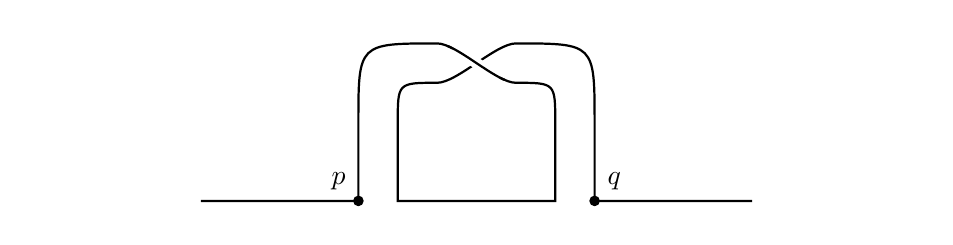
\begin{tikzpicture}
\begin{knot}[clip width = 5, consider self intersections = true]
\clip (-0.2, -0.2) rectangle (11.2, 2.2);
\strand[thick] (2, 0) -- (4, 0) -- (4, 1)
				.. controls +(0, 1) and +(-1, 0) .. (5, 2)
				.. controls +(0.25, 0) and +(-0.25, 0) .. (6, 1.5)
				.. controls +(0.5, 0) and +(0, 0.5) .. (6.5, 1)
				-- (6.5, 0) -- (4.5, 0) -- (4.5, 1)
				.. controls +(0, 0.5) and +(-0.5, 0) .. (5, 1.5)
				.. controls +(0.25, 0) and +(-0.25, 0) .. (6, 2)
				.. controls +(1, 0) and +(0, 1) .. (7, 1)
				-- (7, 0) -- (9, 0);
\end{knot}
\node at (3.75, 0.25) {\contour{white}{$p$}};
\node at (7.25, 0.25) {\contour{white}{$q$}};
\draw[fill = black] (4, 0) circle (0.06);
\draw[fill = black] (7, 0) circle (0.06);
\end{tikzpicture}
\caption{Tracing a band arising from Brunner's construction on a tree. Note that the situation is the same if instead of one twist there are an odd number of twists in $B$.}
\label{fig:tracing-band}
\end{figure}

Contracting this path yields a surface with one band less. By the induction hypothesis the boundary of this is a knot. Thus, so is the boundary of $S$.
\end{proof}

\begin{theorem}
Let $W$ be a Coxeter group. Then $W$ is a Coxeter quotient of a knot if and only if the set $T$ of reflections in $W$ is a single conjugacy class.
\end{theorem}

\begin{proof}
Let $\Gamma$ be the graph of $W$, and let $\Gamma_0$ be the subgraph of $\Gamma$ only consisting of the odd-weighted edges as in Section \ref{subsec:conjugacy-classes}. Since all meridians in a knot group are conjugate it follows that if $\Gamma_0$ is disconnected, then $W$ is not a Coxeter quotient of a knot.

Conversely, if $\Gamma_0$ is connected, apply Brunner's construction to $\Gamma_0$. This is a knot by \ref{lem:tree->knot}. Moreover it has a Coxeter quotient isomorphic to the Coxeter group $\widetilde{W}$ corresponding to the graph $\Gamma_0$ whose non-edges are replaced by edges labeled $\infty$. This group itself has a Coxeter quotient isomorphic to~$W$.
\end{proof}

\section{Torus Knots}\label{sec:torus-knots}
The motto of this section will be that \textit{torus knots tend to admit few Coxeter quotients}. This is evident first in Section \ref{subsec:odd-weights}, where we show that an infinite class of torus knots does not admit any non-trivial Coxeter quotients, further adding to the well-known statement that \textit{knots of determinant one admit poor representation theory}.

\begin{proposition}
Let $p, q$ be positive integers. Then we have that the bridge index of the $(p, q)$-torus knot is $p$. In particular, the $(p, q)$-torus knot does not admit any Coxeter quotients of rank higher than~$p$.
\end{proposition}
%TODO prove

\subsection{Odd Weights}\label{subsec:odd-weights}
As with many things when considering torus knots, the qualitative features as far as Coxeter quotients go depend heavily on the weights $p, q$ of the $(p, q)$-torus knots. The reason for just considering odd weights lies in the fact that if $p$ and $q$ are odd, the $(p, q)$-torus knot has determinant one. To see this, consider the following.
%TODO cite

\begin{theorem}
Let $p, q$ be odd positive integers. Then the Alexander polynomial of $K = T(p, q)$ is
$$\Delta_K(t) = \frac{(t^{pq}-1)(t-1)}{(t^q-1)(t^p-1)}.$$
\end{theorem}

Because the determinant of a knot is its Alexander polynomial evaluated at $-1$, we immediately obtain that $\det T(p, q) = 1$ whenever $p$ and $q$ are odd.

\begin{corollary}
Let $p, q$ be odd. Then the $(p, q)$-torus has determinant one.
\end{corollary}

In Section \ref{subsec:rank-two} we have seen that this implies that torus knots with odd weights do not admit dihedral quotients. This brings us one step closer to the claim that torus knots with odd weights have very few Coxeter quotients. To illustrate our strategies, let us first fix $p = 3$.

\begin{theorem}\label{thm:p=3}
Let $q$ be an odd positive integer such that $q$ has no prime factor less than or equal to~$5$. Then the $(3, q)$-torus knot does not admit any non-trivial Coxeter quotients.
\end{theorem}

Before proving this, we need an easy lemma.

\begin{lemma}
The only irreducible finite Coxeter groups with abelianization $\mathbb{Z}_2$ of rank three are $\mathbb{Z}_2 \times A_5$ and $S_4$.
\end{lemma}

\begin{proof}
This follows directly from the classification of finite irreducible Coxeter groups, see Table \ref{tab:classification}.
\end{proof}

\begin{proof}[Proof of Theorem \ref{thm:p=3}]
It suffices to prove that $K = T(3, q)$ does not admit any rank three Coxeter quotients. Toward a contradiction, suppose $W$ is a Coxeter quotient of $K$ of rank three. Since $K$ is a knot we have that $W$ is irreducible. We will now consider two cases.

First, if $W$ is infinite, then $W$ has trivial center. Let $G = \pi(K)$ and consider the quotient map $\varphi: G \rightarrow W$. Recall that this means that for any meridian $m$ of $K$ we have that $\varphi(m)$ is a reflection in $W$. Since $\varphi$ is surjective we have that the center of $G$ is mapped into the center of $W$, and is thus sent to the identity. Recall that $G$ has a presentation
$$G = \langle a, b \; | \; a^3 = b^q \rangle$$
where $a$ and $b$ are meridian and longitude of the torus on which $K$ lies, respectively. Moreover, the center of $G$ is generated by the element $a^p = b^q$, which is a composition of an odd number of diagram meridians of $K$ since both $p$ and~$q$ are odd. But this is a contradiction: the image of $a^p = b^q$ in $W$ under~$\varphi$ is orientation-preserving because it is the identity, and orientation-reversing because it is the product of an odd number of reflections.

Finally, suppose $W$ is finite. Then $W$ is isomorphic to either $S_4$ or $\mathbb{Z}_2 \times A_5$ since $K$ is a knot. Note that $\varphi(b)$ has order dividing $q$, but by assumption $q$ has no divisor that is also a divisor of the order of $W$, which is either $24 = 2^3 \cdot 3$ or $120 = 2^3 \cdot 3 \cdot 5$.
%There are no infinite ones because $\pi(K)$ has non-trivial center and no finite ones because neither $S_4$ nor $\mathbb{Z}_2 \times A_5$ have elements of order the prime factor greater than or equal to $7$.
\end{proof}

A very similar Theorem is true for $p \geq 5$, as another close look at the classification of finite irreducible Coxeter groups in Table \ref{tab:classification} shows.

\begin{lemma}
No irreducible finite Coxeter group of odd rank $p \geq 5$ has an element of order $q > p$, where~$q$ is prime.
\end{lemma}

\begin{theorem}
Let $5 \leq p < q$ be any odd coprime integers such that $q$ has no prime factor less than or equal to $p$. Then the $(p, q)$-torus knot does not admit any non-trivial Coxeter quotients.
\end{theorem}

\begin{proof}
This is completely analogous to Theorem \ref{thm:p=3}.
\end{proof}

\subsection{Close Weights}
This section contains an upshot showing that some torus knots in fact do have Coxeter quotients, namely the $(n, n + 1)$-torus knots.

\begin{example}[$n=4$]
Consider the braid representation of the $(4, 5)$-torus knot in Figure~\ref{fig:torus45}.

\begin{figure}[ht]
\centering
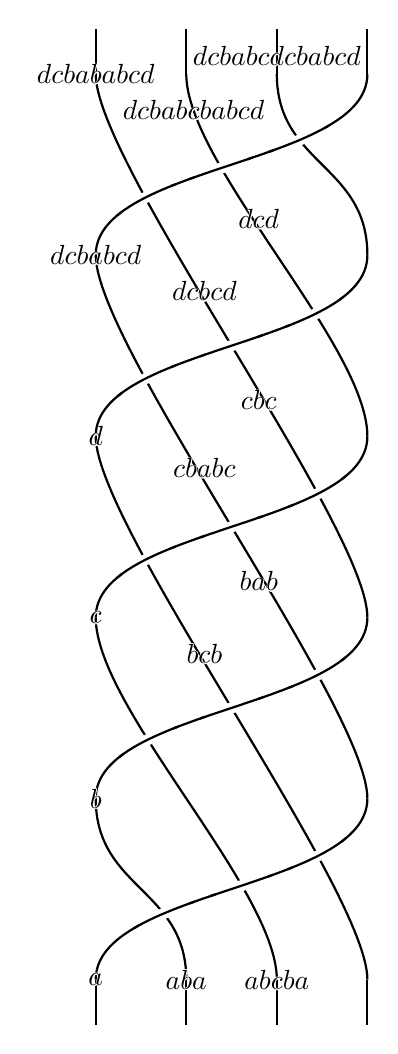
\begin{tikzpicture}[scale = 1.15]
\begin{knot}[clip width = 5, flip crossing/.list = {4, 5,6, 10, 11, 12}]
\strand[thick] (0, -0.5) -- (0, 0);
\strand[thick] (1, -0.5) -- (1, 0);
\strand[thick] (2, -0.5) -- (2, 0);
\strand[thick] (3, -0.5) -- (3, 0);

\strand[thick] (0, 0) .. controls +(0, 1) and +(0, -1) .. (3, 2);
\strand[thick] (1, 0) .. controls +(0, 1) and +(0, -1) .. (0, 2);
\strand[thick] (2, 0) .. controls +(0, 1) and +(0, -1) .. (0, 4);
\strand[thick] (3, 0) .. controls +(0, 1) and +(0, -1) .. (0, 6);

\strand[thick] (0, 2) .. controls +(0, 1) and +(0, -1) .. (3, 4);
\strand[thick] (0, 4) .. controls +(0, 1) and +(0, -1) .. (3, 6);
\strand[thick] (3, 2) .. controls +(0, 1) and +(0, -1) .. (0, 8);
\strand[thick] (3, 4) .. controls +(0, 1) and +(0, -1) .. (0, 10);

\strand[thick] (0, 6) .. controls +(0, 1) and +(0, -1) .. (3, 8);
\strand[thick] (0, 8) .. controls +(0, 1) and +(0, -1) .. (3, 10);

\strand[thick] (3, 6) .. controls +(0, 1) and +(0, -1) .. (1, 10);
\strand[thick] (3, 8) .. controls +(0, 1) and +(0, -1) .. (2, 10);



\strand[thick] (0, 10) -- (0, 10.5);
\strand[thick] (1, 10) -- (1, 10.5);
\strand[thick] (2, 10) -- (2, 10.5);
\strand[thick] (3, 10) -- (3, 10.5);
\end{knot}

\node at (0, 0) {\contour{white}{$a$}};
\node at (0, 2) {\contour{white}{$b$}};
\node at (0, 4) {\contour{white}{$c$}};
\node at (0, 6) {\contour{white}{$d$}};
\node at (0, 8) {\contour{white}{$dcbabcd$}};
\node at (0, 10) {\contour{white}{$dcbababcd$}};

\node at (1.2, 7.6) {\contour{white}{$dcbcd$}};
\node at (1.8, 8.4) {\contour{white}{$dcd$}};
\node at (1.8, 6.4) {\contour{white}{$cbc$}};
\node at (1.8, 4.4) {\contour{white}{$bab$}};
\node at (1.2, 5.65) {\contour{white}{$cbabc$}};
\node at (1.08, 9.6) {\contour{white}{$dcbabcbabcd$}};
\node at (2, 10.2) {\contour{white}{$dcbabcdcbabcd$}};

\node at (1, 0) {\contour{white}{$aba$}};
\node at (1.2, 3.6) {\contour{white}{$bcb$}};
\node at (2, 0) {\contour{white}{$abcba$}};
\end{tikzpicture}
\caption{The case $n = 4$}
\label{fig:torus45}
\end{figure}

Considering the first three strands we obtain a presentation of the reflection quotient of $K$, namely
$$r(K) = \langle a, b, c, d \; | \; adcbababcd, abadcbabcbabcd, abcbadcbabcdcbabcd \rangle^{(2)}.$$
The rules $a \mapsto (1 \; 2)$, $b \mapsto (2 \; 3)$, $c \mapsto (3 \; 4)$, $d \mapsto (4 \; 5)$ extend to a surjective homomorphism $r(K) \rightarrow S_5$, because all relators are mapped to the identity.
\end{example}

\begin{theorem}
Let $n \geq 2$ be an integer. Then the $(n, n+1)$-torus knot admit a Coxeter quotient isomorphic to $S_{n+1}$. In particular, $(n, n+1)$-torus knots are Coxeter.
\end{theorem}

\begin{proof} Similarly as before we consider the braid representation of the $(n, n+1)$-torus knot in Figure \ref{fig:torusnn+1}. The first $n-1$ strands give us the following defining relations.
\begin{itemize}
\setlength\itemsep{0em}
\item $s_1 = s_n \cdots s_1 s_2 s_1 \cdots s_n$
\item $s_1s_2s_1 = s_n \cdots s_1 s_2 s_3 s_2 s_1 \cdots s_n$
\item \dots
\item $s_1 \cdots s_i \cdots s_1 = s_n \cdots s_1 \cdots s_{i+1} \cdots s_1 \cdots s_n$ for $1 \leq i \leq n-1$
\item \dots
\item $s_1 \cdots s_{n-1} \cdots s_1 = s_n \cdots s_1 \cdots s_n \cdots s_1 \cdots s_n$
\end{itemize}
These relations are all satisfied under the map $s_i \mapsto (i \;\;\; i+1)$. To see this, compute 
$$s_{i+1} \cdots s_1 \cdots s_{i+1} \cdots s_1 \cdots s_{i+1} \mapsto (1 \;\; i+1)$$
which is fixed by conjugation with $s_j$ for $j > i$. So the right hand side of the relation is equal to $(1 \; \; i + 1)$. But $s_1 \cdots s_{i-1} \mapsto (1 \; \cdots \; i)$, which conjugates $s_i$ to $(1 \; \; i + 1)$, so the left hand side is also equal to $(1 \; \; i + 1)$. 
\end{proof}

\begin{figure}
\centering
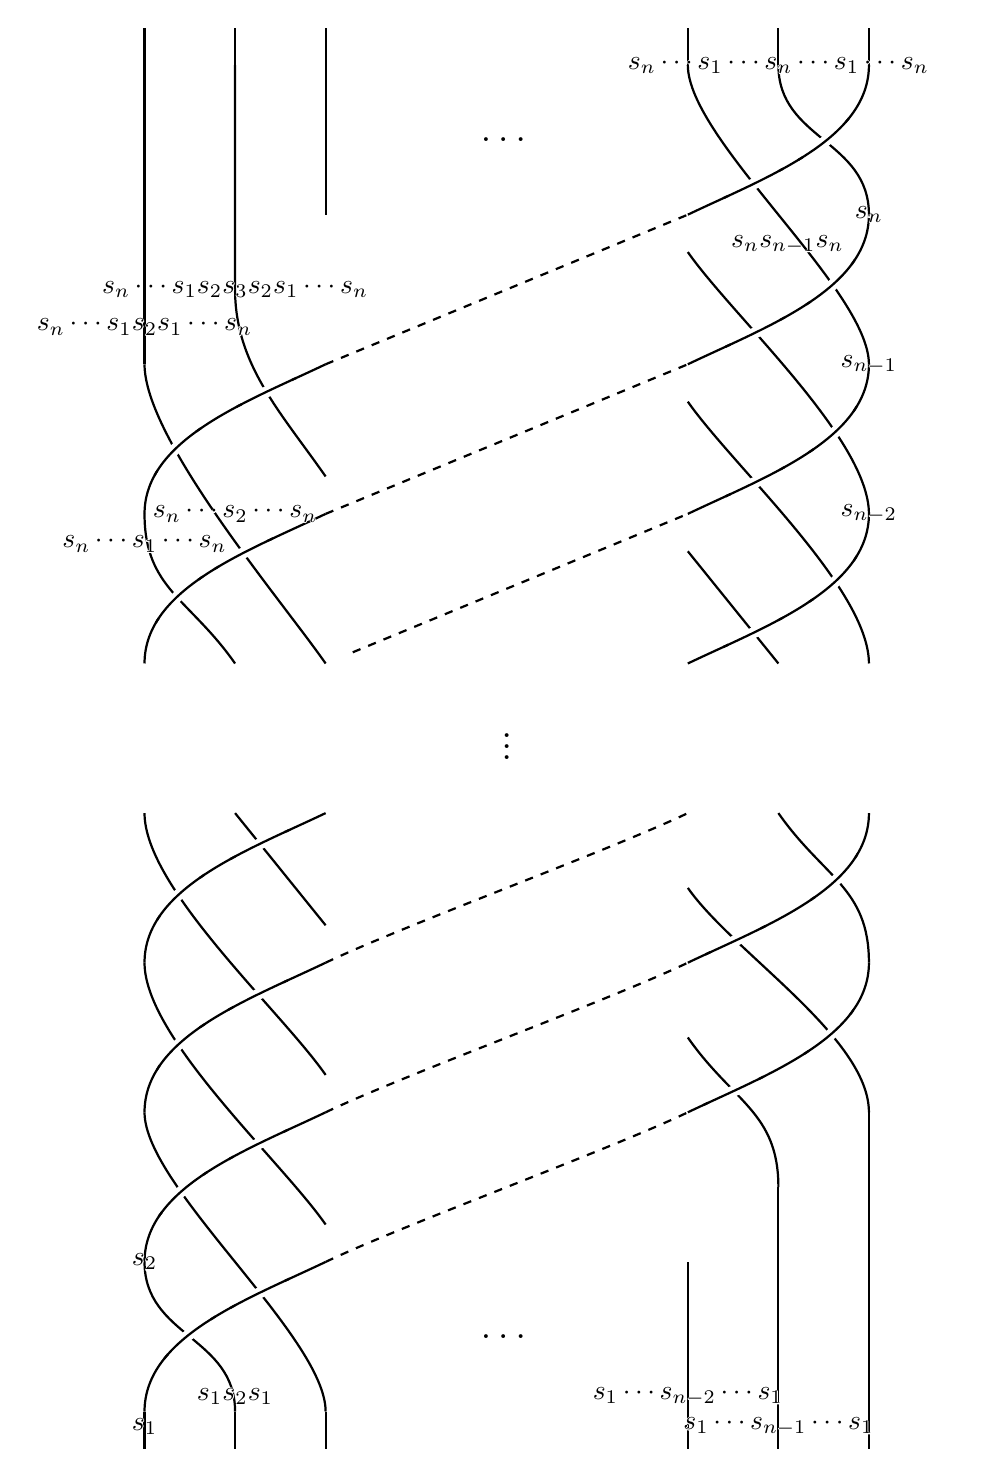
\begin{tikzpicture}[yscale=0.95, xscale=1.15]
\begin{knot}[clip width = 5]
\clip (-1.2, -0.5) rectangle (9.2, 18.5);
\strand[thick] (0, 0) .. controls +(0,1) and +(30:-1) .. (2, 2);
\strand[thick, dashed] (2, 2) .. controls +(30:1) and +(30:-1) .. (6, 4);
\strand[thick] (6, 4) .. controls +(30:1) and +(0, -1) .. (8, 6);
\strand[thick] (1, 0) .. controls +(0, 1) and +(0, -1) .. (0, 2);

\strand[thick] (0, 2) .. controls +(0,1) and +(30:-1) .. (2, 4);
\strand[thick, dashed] (2, 4) .. controls +(30:1) and +(30:-1) .. (6, 6);
\strand[thick] (6, 6) .. controls +(30:1) and +(0, -1) .. (8, 8);
\strand[thick] (2, 0) .. controls +(0, 1) and +(0, -1) .. (0, 4);

\strand[thick] (0, 4) .. controls +(0,1) and +(30:-1) .. (2, 6);
\strand[thick, dashed] (2, 6) .. controls +(30:1) and +(30:-1) .. (6, 8);

\strand[thick] (0, 6) .. controls +(0, 1) and +(30:-1) .. (2, 8);

\strand[thick] (6, 0) -- (6, 2);
\strand[thick] (7, 0) -- (7, 3);
\strand[thick] (7, 3) .. controls +(0, 1) and +(120:-1) .. (6, 5);
\strand[thick] (8, 0) -- (8, 4);
\strand[thick] (8, 4) .. controls +(0, 1) and +(120:-1) .. (6, 7);
\strand[thick] (8, 6) .. controls +(0, 1) and +(120:-1) .. (7, 8);

\strand[thick] (2, 6.5) -- (1, 8);
\strand[thick] (2, 2.5) .. controls +(120:1) and +(0, -1) .. (0, 6);
\strand[thick] (2, 4.5) .. controls +(120:1) and +(0, -1) .. (0, 8);

\strand[thick] (0, 10) .. controls +(0,1) and +(30:-1) .. (2, 12);
\strand[thick, dashed] (2, 12) -- (6, 14);
\strand[thick] (6, 14) .. controls +(30:1) and +(0, -1) .. (8, 16);


\strand[thick] (0, 12) .. controls +(0,1) and +(30:-1) .. (2, 14);
\strand[thick, dashed] (2, 14) -- (6, 16);
\strand[thick] (6, 16) .. controls +(30:1) and +(0, -1) .. (8, 18);
\strand[thick] (1, 10) .. controls +(120:1) and +(0, -1) .. (0, 12);
\strand[thick] (2, 10) .. controls +(120:1) and +(0, -1) .. (0, 14);
\strand[thick] (0, 14) -- (0, 18);

\strand[thick] (2, 12.5) .. controls +(120:1) and +(0,-1) .. (1, 15) -- (1, 18);
\strand[thick] (2, 16) -- (2, 18);

\strand[thick, dashed] (2.3, 10.15) -- (6, 12);
\strand[thick] (6, 12) .. controls +(30:1) and +(0, -1) .. (8, 14);
\strand[thick] (6, 10) .. controls +(30:1) and +(0, -1) .. (8, 12);

\strand[thick] (8, 16) .. controls +(0, 1) and +(0, -1) .. (7, 18);
\strand[thick] (8, 14) .. controls +(0, 1) and +(0, -1) .. (6, 18);
\strand[thick] (8, 12) .. controls +(0, 1) and +(120:-1) .. (6, 15.5);
\strand[thick] (8, 10) .. controls +(0, 1) and +(120:-1) .. (6, 13.5);
\strand[thick] (7, 10) -- (6, 11.5);

%tails
\strand[thick] (0, 18) -- +(0, 0.5);
\strand[thick] (1, 18) -- +(0, 0.5);
\strand[thick] (2, 18) -- +(0, 0.5);
\strand[thick] (6, 18) -- +(0, 0.5);
\strand[thick] (7, 18) -- +(0, 0.5);
\strand[thick] (8, 18) -- +(0, 0.5);

\strand[thick] (0, 0) -- +(0, -0.5);
\strand[thick] (1, 0) -- +(0, -0.5);
\strand[thick] (2, 0) -- +(0, -0.5);
\strand[thick] (6, 0) -- +(0, -0.5);
\strand[thick] (7, 0) -- +(0, -0.5);
\strand[thick] (8, 0) -- +(0, -0.5);
\end{knot}

\node at (4, 1) {\Large{$\dots$}};
\node at (4, 17) {\Large{$\dots$}};
\node at (4, 9) {\Large{$\vdots$}};

\node at (0, -0.2) {\contour{white}{$s_1$}};
\node at (0, 2) {\contour{white}{$s_2$}};
%\node at (0, 4) {\contour{white}{$s_3$}};

\node at (1, 0.2) {\contour{white}{$s_1s_2s_1$}};
%\node at (1, 2) {\contour{white}{$s_2s_3s_2$}};
%\node at(2, 0.2) {\contour{white}{$s_1s_2s_3s_2s_1$}};
\node at (6, 0.2) {\contour{white}{$s_1 \dotsm s_{n-2} \dotsm s_1$}};
\node at (7, -0.2) {\contour{white}{$s_1 \dotsm s_{n-1} \dotsm s_1$}};
%\node at (0, 10) {\contour{white}{$s_n$}};
\node at (8, 14) {\contour{white}{$s_{n-1}$}};
\node at (8, 12) {\contour{white}{$s_{n-2}$}};
%\node at (8, 10) {\contour{white}{$s_{n-3}$}};
%\node at (7.5, 13.6) {\contour{white}{$s_{n-1}s_{n-2}s_{n-1}$}};
%\node at (6.4, 13.2) {\contour{white}{$s_{n-1}s_{n-2}s_{n-3}s_{n-2}s_{n-1}$}};

\node at (8, 16) {\contour{white}{$s_n$}};
\node at (7.1, 15.6) {\contour{white}{$s_ns_{n-1}s_n$}};
\node at (0, 11.6) {\contour{white}{$s_n\dotsm s_1 \dotsm s_n$}};
\node at (1, 12) {\contour{white}{$s_n \dotsm s_2 \dotsm s_n$}};

\node at (0, 14.5) {\contour{white}{$s_n \dotsm s_1 s_ 2 s_ 1 \dotsm s_n$}};
\node at (1, 15) {\contour{white}{$s_n \dotsm s_1 s_ 2 s_3 s_2 s_1 \dotsm s_n$}};
\node at (7, 18) {\contour{white}{$s_n \dotsm s_1 \dotsm s_n \dotsm s_1 \dotsm s_n$}};

\end{tikzpicture}
\caption{The braid representation of the $(n, n+ 1)$-torus knot}
\label{fig:torusnn+1}
\end{figure}

\subsection{Other Weights}
We are nowhere close to understanding what happens in the cases not covered above. For example, the $(3, 5)$- and the $(3, 25)$-torus knots both have a $\mathbb{Z}_2 \times A_5$-quotient. Moreover, all known Coxeter quotients of Torus knots and links are finite, which is not clear from the above arguments.

\newpage
%
%\section{Pretzel Knots}
%\subsection{Preliminaries}
%\subsection{A Coxeter Quotient}
%\begin{theorem}\label{thm:pretzel-links-are-coxeter}
%Pretzel links are Coxeter. 
%\end{theorem}
%
%\begin{proof} First consider the situation of how assigning letters to meridians propagates in 2-braids in Figure \ref{fig:elementary-twists}.
%\begin{figure}[ht]
%\centering
%\begin{minipage}{.35\textwidth}
%\centering
%
%\begin{tikzpicture}[scale = 0.6]
%\begin{knot}[clip width = 5, flip crossing = 2]
%
%\strand[black, thick] (0, 0) .. controls +(0, 1) and +(0, -1) .. (2, 2) .. controls +(0, 1) and +(0, -1) .. (0, 4);
%
%\strand[black, thick] (2, 0) .. controls +(0, 1) and +(0, -1) .. (0, 2) .. controls +(0, 1) and +(0, -1) .. (2, 4);
%
%\strand[black, thick] (0, 6) .. controls +(0, 1) and +(0, -1) .. (2, 8);
%
%\strand[black, thick] (2, 6) .. controls +(0, 1) and +(0, -1) .. (0, 8);
%
%\end{knot}
%
%\node at (1, 4.6) [circle, fill, inner sep=1pt]{};
%\node at (1, 5) [circle, fill, inner sep=1pt]{};
%\node at (1, 5.4) [circle, fill, inner sep=1pt]{};
%
%
%\node at (-1.4, 0) {$x$};
%\node at (3.4, 0) {$y$};
%\node at (-1.4, 2) {$xyx$};
%\node at (-1.4, 4) {$(xy)^2x$};
%\node at (-1.4, 6) {$(xy)^{n-1}x$};
%\node at (-1.4, 8) {$(xy)^nx$};
%\node at (3.4, 8) {$(xy)^{n-1}x$};
%
%\end{tikzpicture}
%
%\end{minipage}%
%\begin{minipage}{.35\textwidth}
%\centering
%\begin{tikzpicture}[scale = 0.6]
%\begin{knot}[clip width = 5, flip crossing/.list = {1, 3}]
%
%\strand[black, thick] (0, 0) .. controls +(0, 1) and +(0, -1) .. (2, 2) .. controls +(0, 1) and +(0, -1) .. (0, 4);
%
%\strand[black, thick] (2, 0) .. controls +(0, 1) and +(0, -1) .. (0, 2) .. controls +(0, 1) and +(0, -1) .. (2, 4);
%
%
%\strand[black, thick] (0, 6) .. controls +(0, 1) and +(0, -1) .. (2, 8);
%
%\strand[black, thick] (2, 6) .. controls +(0, 1) and +(0, -1) .. (0, 8);
%
%\end{knot}
%
%
%\node at (1, 4.6) [circle, fill, inner sep=1pt]{};
%\node at (1, 5) [circle, fill, inner sep=1pt]{};
%\node at (1, 5.4) [circle, fill, inner sep=1pt]{};
%
%\node at(-1.4, 0) {$z$};
%\node at(3.4, 0) {$w$};
%\node at (3.4, 2) {$wzw$};
%\node at (3.4, 4) {$(wz)^2w$};
%\node at (3.4, 6) {$(wz)^{n-1}w$};
%\node at (3.4, 8) {$(wz)^n w$};
%\node at (-1.4, 8) {$(wz)^{n-1}w$};
%
%\end{tikzpicture}
%
%\end{minipage}
%\caption{The relations for 2-braids}
%\label{fig:elementary-twists}
%\end{figure}
%
%Now note that assigning letters of meridians as in the local situation in Figure \ref{fig:local-picture-pretzel-link}, we in fact obtain a generating set of the link group $\pi(P(l_1, \dots, l_k))$.
%
%
%\begin{figure}[ht]
%\centering
%\begin{tikzpicture}
%\draw[ultra thick] (0, -1.5) -- (0, 0) -- (1, 0) -- (1, -1.5);
%\draw[ultra thick] (2, -1.5) -- (2, 0) -- (3, 0) -- (3, -1.5);
%
%\begin{knot}
%\strand[thick] (0.25, 0) .. controls +(0, 0.2) and +(0.2, 0) .. (-1, 0.2);
%\strand[thick] (0.75, 0) .. controls +(0, 0.2) and +(0, 0.2) .. (2.25, 0);
%\strand[thick] (2.75, 0) .. controls +(0, 0.2) and +(0.2, 0) .. (4, 0.2);
%\end{knot}
%
%\node at (0, 0.4) {$x$};
%\node at (1, 0.4) {$y$};
%\node at (2, 0.4) {$z$};
%\node at (3, 0.4) {$w$};
%
%\node at (0.5, -0.75) {$a$};
%\node at (2.5, -0.75) {$b$};
%\end{tikzpicture}
%
%\caption{A local picture}
%\label{fig:local-picture-pretzel-link}
%\end{figure}
%
%Putting these 2-braids together as in Figure \ref{fig:local-picture-pretzel-link} we obtain the following relation in the knot group from the requirement that $y = z$ according as to whether $a$ and $b$ are positive or negative:
%
%\begin{itemize}
%\setlength\itemsep{0em}
%\item If both $a$ and $b$ are positive, then we obtain $(xy)^{a-1}x = (yw)^by.$
%\item If $a$ is positive and $b$ is negative, we obtain $(xy)^{a-1}x = (wy)^{-b+1}w$.
%\item If $a$ is negative and $b$ is positive, we obtain $(yx)^{-a}y = (yw)^b y$.
%\item If both $a$ and $b$ are negative, then we obtain $(yx)^{-a}y = (wy)^{-b+1}w$.
%\end{itemize}
%
%All these relations follow from the Coxeter relations $(xy)^{|a|} = (yw)^{|b|} = 1$. Assigning generators as in Figure \ref{fig:local-picture-pretzel-link} we get a quotient of the desired form.
%\end{proof}
%
%\begin{corollary}
%Pretzel links satisfy the meridional rank conjecture.
%\end{corollary}
%%TODO cite
%
%\begin{proof}
%This is just Corollary \ref{cor:coxeter-links-meridional-rank}.
%\end{proof}
%
%It might be worth pointing out that the explicit Coxeter quotient obtained is described by the matrix
%
%$$
%\renewcommand\arraystretch{1.2}
%M = \left( \begin{matrix}
%1 & l_1 & \infty & \cdots & \cdots &\cdots & \infty & l_n \\
%l_1 & 1 & l_2 & \infty & \cdots & \cdots & \infty & \infty \\
%\infty & l_2 & 1 & l_3 & \infty &\cdots & \infty & \infty \\
%\vdots & \infty  & l_3 & 1 & \ddots & \ddots & \vdots & \vdots \\
%\vdots & \vdots & \infty & \ddots & \ddots & \ddots & \infty & \vdots \\
%\vdots & \vdots & \vdots & \ddots &\ddots & 1 & \l_{n-2} & \infty \\
%\infty & \infty & \infty & \cdots & \infty & l_{n-2} & 1 & l_{n-1} \\
%l_n & \infty & \infty & \cdots & \cdots & \infty  & l_{n-1} & 1
%\end{matrix} \right).$$
%
%\newpage




\newpage
\section{Ribbon Theory}
\subsection{Ribbon and Slice Disks}\label{subsec:ribbons}
A \textit{ribbon disk} is a smooth immersion $D^2 \rightarrow S^3$ of a disk $D^2$ that only has single and double points such that it becomes an embedding after removing finitely many intervals from the interior of $D^2$. A \textit{ribbon knot} is a knot that bounds a ribbon disk.

This can be visualized as follows. Let us call connected components of double points of a ribbon disk \textit{ribbon singularities}. Then a ribbon singularity looks like a slit cut into the interior of the ribbon in order to allow another part of the ribbon to pass through, see Figure \ref{fig:ribbon-singularity}. The singularity in Figure \ref{fig:not-ribbon-singularity} is not a ribbon singularity because the slit that we would need to cut involves a point on the boundary of the ribbon.

\begin{figure}[htb]
\centering
\begin{minipage}{0.5\textwidth}
\centering
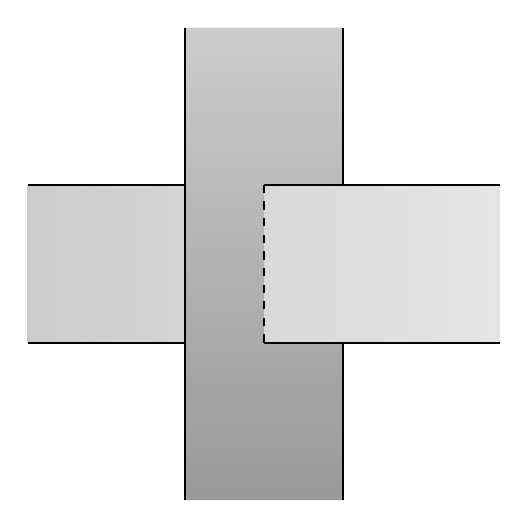
\begin{tikzpicture}
\clip (0, -2) rectangle (6, 4);
\shade[left color=black!20, right color = black!10] (0, 0) rectangle (6, 2);
\shade[bottom color=black!40, top color = black!20] (2, -2) -- (2, 4) -- (4, 4) -- (4, 2) -- (3, 2) -- (3, 0) -- (4, 0) -- (4, -2) -- (2, -2);
\draw[thick] (2, 0) -- (0, 0);
\draw[thick] (0, 2) -- (2, 2);
\draw[thick] (3, 2) -- (6, 2);
\draw[thick] (6, 0) -- (3, 0);
\draw[thick, dashed] (3, 0) -- (3, 2);
\draw[thick] (4, 2) -- (4, 4);
\draw[thick] (2, 4) -- (2, -2);
\draw[thick] (4, -2) -- (4, 0);
\end{tikzpicture}
\caption{A ribbon singularity}
\label{fig:ribbon-singularity}
\end{minipage}%
\begin{minipage}{0.5\textwidth}
\centering
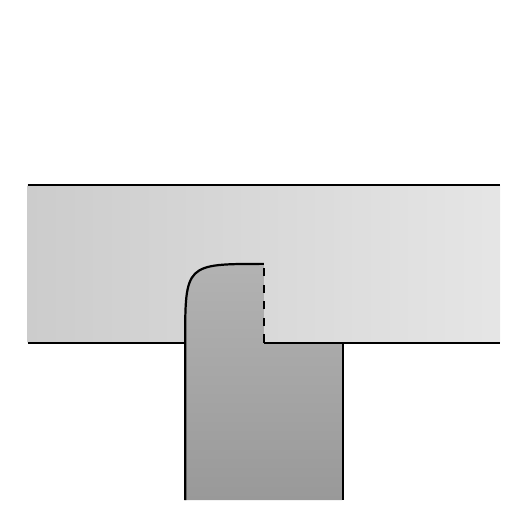
\begin{tikzpicture}
\clip (0, -2) rectangle (6, 4);
\shade[left color=black!20, right color = black!10] (0, 0) rectangle (6, 2);
\shade[bottom color=black!40, top color = black!30] (2, -2) -- (2, 0) .. controls +(0, 1) and +(-1, 0) .. (3, 1) -- (3, 0) -- (4, 0) -- (4, -2) -- (2, -2);

\draw[thick] (2, 0) -- (0, 0);
\draw[thick] (0, 2) -- (6, 2);
\draw[thick] (3, 0) -- (6, 0);
\draw[thick, dashed] (3, 0) -- (3, 1);
\draw[thick] (2, -2) -- (2, 0) .. controls +(0, 1) and +(-1, 0) .. (3, 1);
\draw[thick] (4, -2) -- (4, 0);
\end{tikzpicture}
\caption{Not a ribbon singularity}
\label{fig:not-ribbon-singularity}
\end{minipage}
\end{figure}

We start by considering a particular family of ribbon knots.

\begin{theorem}\label{thm:connected-sum-ribbon}
Let $K$ be any knot and $\bar{K}$ its mirror image. Then the connected sum $K\#\bar{K}$ is a ribbon knot.
\end{theorem}

\begin{proof}[Proof sketch]
Suppose $P$ is the plane such that orthogonal reflection in $P$ throws the knot $K\#\bar{K}$ onto itself. In the example in Figure \ref{fig:connected-sum-figure-8} the plane $P$ is represented by the dashed line. 

\begin{figure}[htb]
\centering
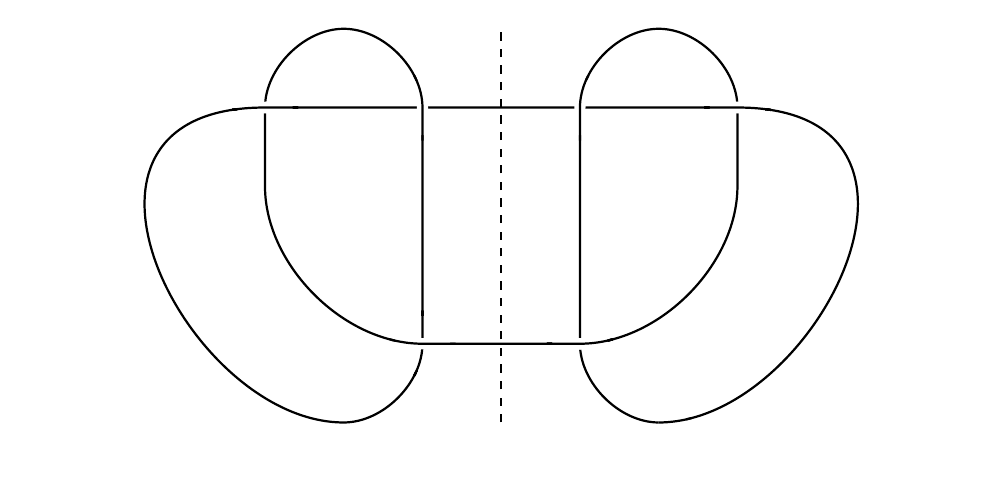
\begin{tikzpicture}
%\clip (-4, -2) rectangle (4, 5);
\begin{knot}[clip width = 5, consider self intersections = true, 
ignore endpoint intersections=false,
%draft mode = crossings,
flip crossing/.list = {4, 15, 9}
]
\strand[thick] (2, 0) .. controls +(2, 0) and +(3, 0) ..
	(3, 4) --
	(-3, 4) .. controls +(-3, 0) and +(-2, 0) ..
	(-2, 0) .. controls +(0.5, 0) and +(0, -0.5) ..
	(-1, 1) -- 
	(-1, 4) .. controls +(0, 0.5) and +(0.5, 0) ..
	(-2, 5) .. controls +(-0.5, 0) and +(0, 0.5) ..
	(-3, 4) --
	(-3, 3) .. controls +(0, -1) and +(-1, 0) ..
	(-1, 1) -- 
	(1, 1) .. controls +(1, 0) and +(0, -1) ..
	(3, 3) --
	(3, 4) .. controls +(0, 0.5) and +(0.5, 0) ..
	(2, 5) .. controls +(-0.5, 0) and +(0, 0.5) ..
	(1, 4) -- 
	(1, 1) .. controls +(0, -0.5) and +(-0.5, 0) ..
	(2, 0);
\end{knot}
\draw[thick, dashed] (0, 0) -- (0, 5);
\end{tikzpicture}
\caption{The connected sum of the Trefoil with its mirror image}
\label{fig:connected-sum-figure-8}
\end{figure}

Now connect corresponding points on the knot by straight lines perpendicular to $P$. By a general position argument arising from the observation that projecting $K\#\bar{K}$ onto $P$ is an immersed interval, the surface formed in this way is a ribbon disk.
\end{proof}

\begin{example}
Figure \ref{fig:ribbon-trefoil-mirror-trefoil} shows the result of applying the procedure in the proof of Theorem \ref{thm:connected-sum-ribbon} to the Trefoil knot.

\begin{figure}[htb]
\centering
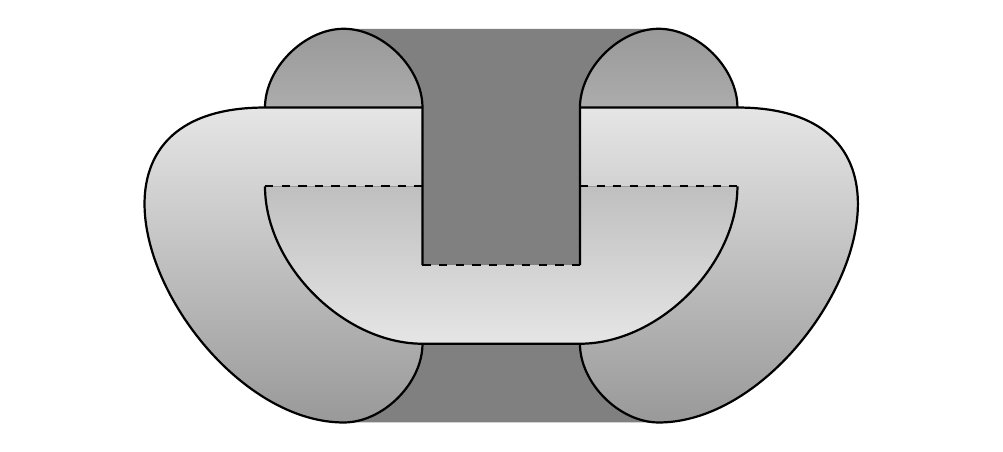
\begin{tikzpicture}
\fill[%pattern = north west lines
		color=black!50]
	(-2, 5) -- 
	(2, 5) .. controls +(-0.5, 0) and +(0, 0.5) ..
	(1, 4) -- 
	(1, 1) .. controls +(0, -0.5) and +(-0.5, 0) ..
	(2, 0) --
	(-2, 0) .. controls +(0.5, 0) and +(0, -0.5) ..
	(-1, 1) --
	(-1, 4) .. controls +(0, 0.5) and +(0.5, 0) ..
	(-2, 5);
	
\fill[color = white] (-1, 1) rectangle (1, 2);

\fill[top color = black!40, bottom color = black!10] 
	(-2, 5) .. controls +(-0.5, 0) and +(0, 0.5) ..
	(-3, 4) --
	(-3, 3) .. controls +(0, -1) and +(-1, 0) ..
	(-1, 1) -- 
	(1, 1) .. controls +(1, 0) and +(0, -1) ..
	(3, 3) -- 
	(3, 4) .. controls +(0, 0.5) and +(0.5, 0) ..
	(2, 5) .. controls +(-0.5, 0) and +(0, 0.5) ..
	(1, 4) --
	(1, 2) --
	(-1, 2) --
	(-1, 4) .. controls +(0, 0.5) and +(0.5, 0) ..
	(-2, 5);
	
\fill[bottom color = black!40, top color = black!10]
	(2, 0) .. controls +(2, 0) and +(3, 0) ..
	(3, 4) -- 
	(1, 4) --
	(1, 3) --
	(3, 3) --
	(3, 3) .. controls +(0, -1) and +(1, 0) ..
	(1, 1) .. controls +(0, -0.5) and +(-0.5, 0) ..
	(2, 0);
	
\fill[bottom color = black!40, top color = black!10]
	(-2, 0) .. controls +(-2, 0) and +(-3, 0) ..
	(-3, 4) -- 
	(-1, 4) --
	(-1, 3) --
	(-3, 3) --
	(-3, 3) .. controls +(0, -1) and +(-1, 0) ..
	(-1, 1) .. controls +(0, -0.5) and +(0.5, 0) ..
	(-2, 0);
	
\draw[thick] (1, 1) .. controls +(0, -0.5) and +(-0.5, 0) ..
	(2, 0) .. controls +(2, 0) and +(3, 0) ..
	(3, 4) --
	(1, 4);
	
\draw[thick] (-1, 1) .. controls +(0, -0.5) and +(0.5, 0) ..
	(-2, 0) .. controls +(-2, 0) and +(-3, 0) ..
	(-3, 4) --
	(-1, 4);
	
\draw[thick] (-3, 3) .. controls +(0, -1) and +(-1, 0) ..
	(-1, 1) -- 
	(1, 1)  .. controls +(1, 0) and +(0, -1) ..
	(3, 3);
	
\draw[thick] (-3, 4) .. controls +(0, 0.5) and +(-0.5, 0) ..
	(-2, 5) .. controls +(0.5, 0) and +(0, 0.5) ..
	(-1, 4) --
	(-1, 2);
	
\draw[thick] (3, 4) .. controls +(0, 0.5) and +(0.5, 0) ..
	(2, 5) .. controls +(-0.5, 0) and +(0, 0.5) ..
	(1, 4) --
	(1, 2);

\draw[thick, dashed] (-1, 2) -- (1, 2);
\draw[thick, dashed] (-3, 3) -- (-1, 3);
\draw[thick, dashed] (1, 3) -- (3, 3);

\end{tikzpicture}
\caption{A ribbon disk for the connected sum of the Trefoil with its mirror image}
\label{fig:ribbon-trefoil-mirror-trefoil}
\end{figure}
\end{example}

There is a related notion concerning four-dimensional properties of knots. It goes as follows. We interpret $S^3$ as the boundary of the unit disk $D^4$ in four-dimensional euclidean space. A \textit{slice disk} is a smooth embedding of a disk $D^2$ into $D^4$ whose boundary $S^1$ is mapped into $S^3$, and whose interior~$B^2$ is mapped into the interior $B^4$ of $D^4$. More concisely, a slice disk is a smooth embedding of the pair~$(B^2, S^1)$ into the pair $(B^4, S^3)$. A knot that is the boundary of a slice disk is called a \textit{slice knot}.

\begin{theorem}\label{thm:ribbon-are-slice}
All ribbon knots are slice knots.
\end{theorem}

\begin{proof}[Proof sketch]
Let $f: D^2 \rightarrow S^3$ be the ribbon disk. We are going to add a height coordinate to $f$ as follows. Take disjoint neighborhoods of the slits that need to be removed from $D^2$ in order for $f$ to become an embedding. Now just add a bump function to these neighborhoods.

This procedure is schematically indicated in Figure \ref{fig:ribbon-knots-are-slice}. More distance from the boundary corresponds to a brighter color, and the slits we were about to cut away are dashed. The increase in brightness up until the inner large circle is to make sure that no part of the interior $B^2$ of $D^2$ is mapped to $S^3$.

\begin{figure}[htb]
\centering
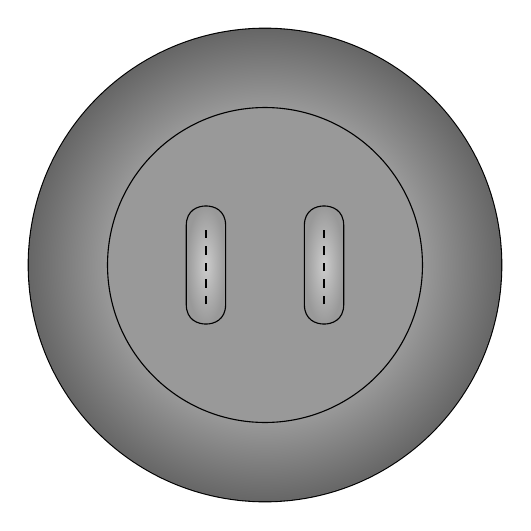
\begin{tikzpicture}
\draw[thick] (0, 0) circle (3);
\fill[outer color = black!60, inner color = white] (0, 0) circle (3);
\fill[color = black!40] (0, 0) circle (2);
\draw (0, 0) circle (2);
\filldraw[outer color = black!40, inner color=black!20] 
	(-0.75, -0.75) .. controls +(0.1, 0) and +(0, -0.2) ..
	(-0.5, -0.5) --
	(-0.5, 0.5) .. controls +(0, 0.2) and +(0.1, 0) ..
	(-0.75, 0.75) .. controls +(-0.1, 0) and +(0, 0.2) ..
	(-1, 0.5) -- 
	(-1, -0.5) .. controls +(0, -0.2) and +(-0.1, 0) ..
	(-0.75, -0.75);
\filldraw[outer color = black!40, inner color=black!20] 
	(0.75, -0.75) .. controls +(-0.1, 0) and +(0, -0.2) ..
	(0.5, -0.5) --
	(0.5, 0.5) .. controls +(0, 0.2) and +(-0.1, 0) ..
	(0.75, 0.75) .. controls +(0.1, 0) and +(0, 0.2) ..
	(1, 0.5) -- 
	(1, -0.5) .. controls +(0, -0.2) and +(0.1, 0) ..
	(0.75, -0.75);
\draw[thick, dashed] (-0.75, -0.5) -- (-0.75, 0.5);
\draw[thick, dashed] (0.75, -0.5) -- (0.75, 0.5);
\end{tikzpicture}
\caption{The disk $D^2$ with some slits with indications how to get an embedding into $D^4$}
\label{fig:ribbon-knots-are-slice}
\end{figure}

Every step we did could have been done smoothly. We have thus constructed a slice disk from a ribbon disk.
\end{proof}

\subsection{The Ribbon Disk Group}
%From now on, let us think of ribbons as slice disks whose associated height function has no local maxima in the interior. Note that given a ribbon disk in $S^3$ we can construct such a slice disk as in the proof of Theorem \ref{thm:ribbon-are-slice}. Conversely, projecting a ribbon disk onto $S^3$ will yield what was called a ribbon disk in Section \ref{subsec:ribbons}.

As with a link group, the \textit{slice disk group} $\pi(S)$ of a slice disk $S$ in $D^4$ is the fundamental group of its complement in $D^4$. If the slice disk is in fact a ribbon $R$, then $\pi(R)$ is called its ribbon group. We define the ribbon group of a ribbon in $S^3$ to be the ribbon group of its embedding into $D^4$ as in the proof of Theorem \ref{thm:ribbon-are-slice}. In this section, we are going to give an algorithm to compute ribbon groups.

\begin{algo}[Computing Ribbon Groups]\label{alg:ribbon-groups}
Let $R$ be a ribbon in $S^3$ with boundary $K$. We will construct a presentation of $\pi(R)$ and a surjective homomorphism $\pi(K) \rightarrow \pi(R)$. Let $R'$ be $R$ with disk neighborhoods of the slits removed. Consider the diagram meridians $s_i$ of $K$ in $S^3$. This will be our generating set. The first set of relations will be the Wirtinger relations of $K$. Assuming correctness of our procedure, it is already clear at this point that $\pi(K)$ will surject onto $\pi(R)$.

The next set of relations is a little bit more subtle. Consider a neighborhood of $R'$ diffeomorphic to~$(D^2 \times I) \setminus D'$, were $D'$ is a standardly embedded disk with $n$ disjoint smaller disks removed. Here, $n$ is the number of ribbon singularities. Figure \ref{fig:an-interesting-curve} depicts the single generating curve in the case $n = 2$. In general we need to consider $n-1$ such curves. Let $\varphi: \mathbb{R}^3 \setminus D' \rightarrow S^3 \setminus K$ be said diffeomorphism composed with the inclusion map. Then $\varphi$ induces a homomorphism $\varphi_*: \pi_1(S^3 \setminus D') \rightarrow \pi_1(K)$. For each generator $\gamma$ of $\pi_1(S^3 \setminus D')$, add the relation $\varphi_*(\gamma) = 1$. We will call these relations the \textit{through-slit relations}.

Finally, consider the inclusion $\iota: S^3 \setminus R' \rightarrow S^3 \setminus L$, where $L$ is the boundary of the ribbon slits. Note that $L$ is a trivial link of $n$ components, where $n$ is the number of ribbon singularities. This induces a homomorphism $\iota_*: \pi_1(S^3 \setminus R') \rightarrow \pi(L)$, where $\pi(L)$ is a free group on $n$ generators. Add the relations $s = t$ for any two meridians $s, t$ that get mapped to the same element in $\pi(L)$ under $\iota_*$. These relations are called the \textit{same-slit relations}.
\end{algo}

\begin{theorem}\label{thm:ribbon-algorithm}
The ribbon group algorithm \textup{(Procedure \ref{alg:ribbon-groups})} yields a presentation of the ribbon group.

\end{theorem}
\begin{figure}[htb]
\centering
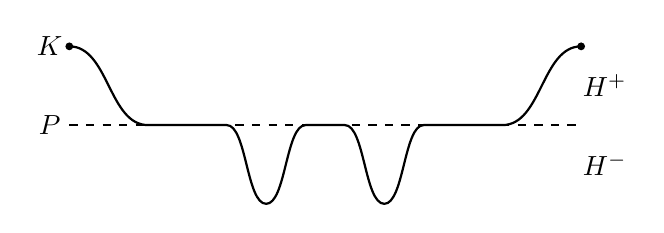
\begin{tikzpicture}
\draw[thick] (0, 0) .. controls +(0.5, 0) and +(-0.5, 0) .. (1,-1) -- (2, -1) .. controls +(0.25, 0) and +(-0.25, 0) .. (2.5, -2) .. controls +(0.25, 0) and +(-0.25, 0) .. (3, -1) -- (3.5, -1) .. controls +(0.25, 0) and +(-0.25, 0) .. (4, -2) .. controls +(0.25, 0) and +(-0.25, 0) .. (4.5, -1)  -- (5.5, -1) .. controls +(0.5, 0) and +(-0.5, 0) .. (6.5, 0);
\draw[thick, dashed] (0, -1) -- (6.5, -1);
\node at (0, 0) [circle, fill, inner sep=1pt]{};
\node at (6.5, 0) [circle, fill, inner sep=1pt]{};
\node at (-0.25, 0) {$K$};
\node at (-0.25, -1) {$P$};
\node at (6.8, -0.5) {$H^+$};
\node at (6.8, -1.5) {$H^-$};
\end{tikzpicture}
\caption{A slice of the ribbon disk complement}
\label{fig:van-kampen-ribbon-complement}
\end{figure}

\begin{proof}[Proof sketch]
Similar to the proof of the Wirtinger Theorem, Theorem \ref{thm:wirtinger-thm}, we apply van Kampen's Theorem to a particular embedding of our ribbon disk, namely the one constructed in the proof of Theorem \ref{thm:ribbon-are-slice}. This time we choose the three-sphere $P$ given by the height of the medium-gray disk in Figure~\ref{fig:ribbon-knots-are-slice}. Again, we consider the half spaces $H^+$ above $P$ and $H^-$ below $P$. In Figure \ref{fig:van-kampen-ribbon-complement}, the neighborhoods of the minima below $P$ are actually small neighbourhoods of the slits.

Note that to obtain $P$ we remove the neighborhoods of the slits from the ribbon, and then remove this from $S^3$. This looks something like what is depicted in Figure \ref{fig:ribbon-nbhds-of-slits-removed}. Consider the curve $\gamma$ described in the procedure, depicted in Figure \ref{fig:an-interesting-curve} for the case $n = 2$ before applying $\varphi$, passing through both slits but not around the boundary. In other words, $\gamma$ is not null-homotopic in $P$ but it is null-homotopic in the knot complement.

\begin{figure}[htb]
\centering
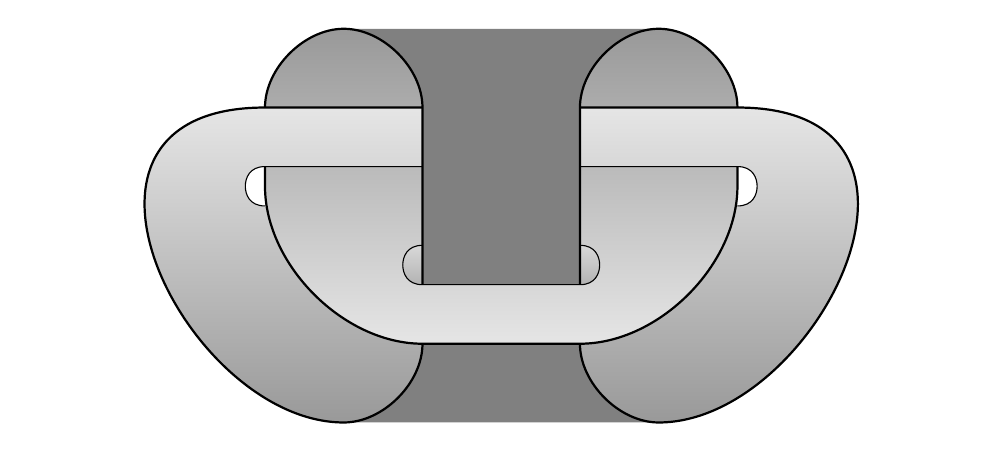
\begin{tikzpicture}
\fill[%pattern = north west lines
		color = black!50]
	(-2, 5) -- 
	(2, 5) .. controls +(-0.5, 0) and +(0, 0.5) ..
	(1, 4) -- 
	(1, 1) .. controls +(0, -0.5) and +(-0.5, 0) ..
	(2, 0) --
	(-2, 0) .. controls +(0.5, 0) and +(0, -0.5) ..
	(-1, 1) --
	(-1, 4) .. controls +(0, 0.5) and +(0.5, 0) ..
	(-2, 5);
	
\fill[top color = black!40, bottom color = black!10] 
	(-2, 5) .. controls +(-0.5, 0) and +(0, 0.5) ..
	(-3, 4) --
	(-3, 3) .. controls +(0, -1) and +(-1, 0) ..
	(-1, 1) -- 
	(1, 1) .. controls +(1, 0) and +(0, -1) ..
	(3, 3) -- 
	(3, 4) .. controls +(0, 0.5) and +(0.5, 0) ..
	(2, 5) .. controls +(-0.5, 0) and +(0, 0.5) ..
	(1, 4) --
	(1, 1.75) --
	(-1, 1.75) --
	(-1, 4) .. controls +(0, 0.5) and +(0.5, 0) ..
	(-2, 5);
	
\fill[bottom color = black!40, top color = black!10]
	(2, 0) .. controls +(2, 0) and +(3, 0) ..
	(3, 4) -- 
	(1, 4) --
	(1, 3.25) --
	(3, 3.25) --
	(3, 3) .. controls +(0, -1) and +(1, 0) ..
	(1, 1) .. controls +(0, -0.5) and +(-0.5, 0) ..
	(2, 0);
	
\fill[bottom color = black!40, top color = black!10]
	(-2, 0) .. controls +(-2, 0) and +(-3, 0) ..
	(-3, 4) -- 
	(-1, 4) --
	(-1, 3.25) --
	(-3, 3.25) --
	(-3, 3) .. controls +(0, -1) and +(-1, 0) ..
	(-1, 1) .. controls +(0, -0.5) and +(0.5, 0) ..
	(-2, 0);

\fill[bottom color=black!30, top color=black!15] 
	(-1, 2.25) .. controls +(-0.2, 0) and +(0, 0.1) ..
	(-1.25, 2) .. controls +(0, -0.1) and +(-0.2, 0) ..
	(-1, 1.75) -- (-1, 2.25);
\fill[bottom color=black!30, top color=black!15]
	(1, 1.75) .. controls +(0.2, 0) and +(0, -0.1) ..
	(1.25, 2) .. controls +(0, 0.1) and +(0.2, 0) ..
	(1, 2.25) -- (1, 1.75);	
	
\fill[color=white]
	(-3, 3.25) .. controls +(-0.2, 0) and +(0, 0.1) ..
	(-3.25, 3) .. controls +(0, -0.1) and +(-0.2, 0) ..
	(-3, 2.75);
\fill[color=white]
	(3, 3.25) .. controls +(0.2, 0) and +(0, 0.1) ..
	(3.25, 3) .. controls +(0, -0.1) and +(0.2, 0) ..
	(3, 2.75);
	
\draw (-1, 2.25) .. controls +(-0.2, 0) and +(0, 0.1) ..
	(-1.25, 2) .. controls +(0, -0.1) and +(-0.2, 0) ..
	(-1, 1.75) -- 
	(1, 1.75) .. controls +(0.2, 0) and +(0, -0.1) ..
	(1.25, 2) .. controls +(0, 0.1) and +(0.2, 0) ..
	(1, 2.25);

\draw (-1, 3.25) -- 
	(-3, 3.25) .. controls +(-0.2, 0) and +(0, 0.1) ..
	(-3.25, 3) .. controls +(0, -0.1) and +(-0.2, 0) ..
	(-3, 2.75);
\draw (1, 3.25) -- 
	(3, 3.25) .. controls +(0.2, 0) and +(0, 0.1) ..
	(3.25, 3) .. controls +(0, -0.1) and +(0.2, 0) ..
	(3, 2.75);
	
\draw[thick] (1, 1) .. controls +(0, -0.5) and +(-0.5, 0) ..
	(2, 0) .. controls +(2, 0) and +(3, 0) ..
	(3, 4) --
	(1, 4);
	
\draw[thick] (-1, 1) .. controls +(0, -0.5) and +(0.5, 0) ..
	(-2, 0) .. controls +(-2, 0) and +(-3, 0) ..
	(-3, 4) --
	(-1, 4);
	
\draw[thick] (-3, 3.25) -- (-3, 3) .. controls +(0, -1) and +(-1, 0) ..
	(-1, 1) -- 
	(1, 1)  .. controls +(1, 0) and +(0, -1) ..
	(3, 3) -- (3, 3.25);
	
\draw[thick] (-3, 4) .. controls +(0, 0.5) and +(-0.5, 0) ..
	(-2, 5) .. controls +(0.5, 0) and +(0, 0.5) ..
	(-1, 4) --
	(-1, 1.75);
	
\draw[thick] (3, 4) .. controls +(0, 0.5) and +(0.5, 0) ..
	(2, 5) .. controls +(-0.5, 0) and +(0, 0.5) ..
	(1, 4) --
	(1, 1.75);
\end{tikzpicture}
\caption{A ribbon disk without neighborhoods of the slits}
\label{fig:ribbon-nbhds-of-slits-removed}
\end{figure}



\begin{figure}[htb]
\centering
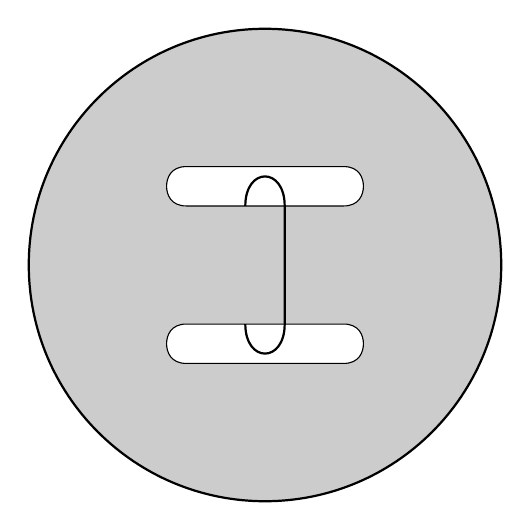
\begin{tikzpicture}
\fill[color = black!20] (0, 0) circle (3);
\draw[thick] (0, 0) circle (3);
\draw[fill = white] 
	(-1.25, -1) .. controls +(0, 0.1) and +(-0.2, 0) ..
	(-1, -0.75) --
	(1, -0.75) .. controls +(0.2, 0) and +(0, 0.1) ..
	(1.25, -1) .. controls +(0, -0.1) and +(0.2, 0) ..
	(1, -1.25) --
	(-1, -1.25) .. controls +(-0.2, 0) and +(0, -0.1) ..
	(-1.25, -1);
\draw[fill = white] 
	(-1.25, 1) .. controls +(0, -0.1) and +(-0.2, 0) ..
	(-1, 0.75) --
	(1, 0.75) .. controls +(0.2, 0) and +(0, -0.1) ..
	(1.25, 1) .. controls +(0, 0.1) and +(0.2, 0) ..
	(1, 1.25) --
	(-1, 1.25) .. controls +(-0.2, 0) and +(0, 0.1) ..
	(-1.25, 1);
\draw[thick] 
	(-0.25, -0.75) .. controls +(0, -0.5) and +(0, -0.5) ..
	(0.25, -0.75) --
	(0.25, 0.75) .. controls +(0, 0.5) and +(0, 0.5) ..
	(-0.25, 0.75);
\end{tikzpicture}
\caption{The curve $\gamma$ passing through two slits}
\label{fig:an-interesting-curve}
\end{figure}

Note that $\pi_1(H^-)$ is the free group generated by the image of $\varphi$. This is because every curve can be assumed to be contained in the interior of $H^-$ with a sole exception for the base point, and because the interior of $H^-$ retracts onto the trivial link $L$ on $n$ components. Moreover, the fundamental group~$\pi_1(P)$ is is generated by diagram meridians and $n-1$ paths like the image of the one in Figure~\ref{fig:an-interesting-curve} under $\varphi$. Finally, since $H^+$ deformation retracts onto $S^3 \setminus K$, we have that $\pi_1(H^+)$ is isomorphic to~$\pi_1(K)$ via the inclusion induced isomorphism.

Now each diagram meridian in $\pi(K)$ that is the image of a curve in $S^3 \setminus R'$ is mapped to itself in~$\pi_1(H^+)$ and to a generator of $\pi_1(H^-)$. Moreover, the curves $\gamma$ as in Figure \ref{fig:an-interesting-curve} are null-homotopic in the knot group $\pi(K)$, so they identify all generators of $\pi_1(H^-)$ that pass through the same ribbon slit when applying van Kampen's Theorem. This covers all relations discussed in the procedure.
\end{proof}

In summary, our procedure goes as follows. First, write down a Wirtinger presentation for the knot. Then, the through-slit relations are the relations induced by null-homotopic curves passing through ribbon slits. Finally, the same-slit relations are the relations identifying meridians passing through the same ribbon slits.

\begin{example}[Connected Sum of the Trefoil With its Mirror Image]\label{ex:square-knot-ribbon}
Consider the generating assignment of curves of $\pi(K)$ in Figure \ref{fig:meridians-of-trefoil-sum-trefoil}. This yields a presentation of the fundamental group of the complement of $K$ with generators $a$, $b$ and $b'$ satisfying Wirtinger relations
$aba = bab \,\text{ and }\, ab'a = b'ab'.$

\begin{figure}[htb]
\centering
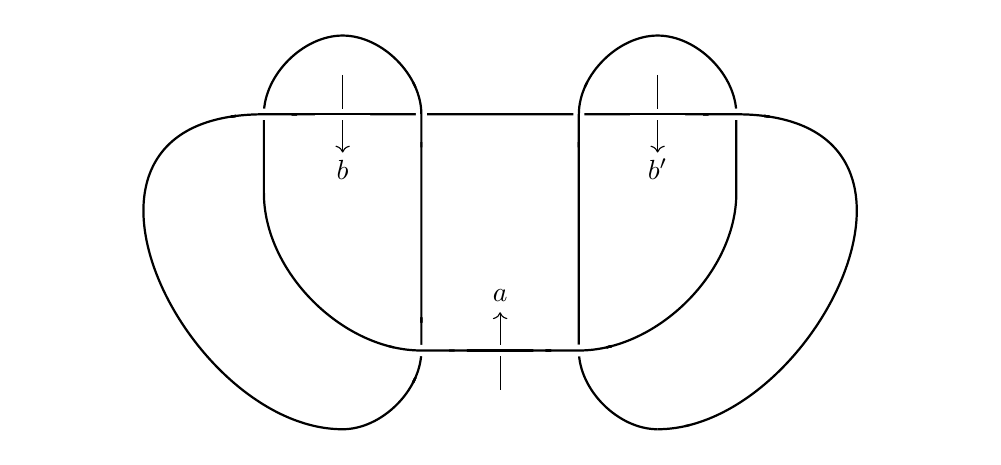
\begin{tikzpicture}
\clip (-6, -0.1) rectangle (6, 5.1);
\begin{knot}[clip width = 5, consider self intersections = true, 
ignore endpoint intersections=false,
%draft mode = crossings,
flip crossing/.list = {4, 17, 9}
]
\strand[thick] (2, 0) .. controls +(2, 0) and +(3, 0) ..
	(3, 4) --
	(-3, 4) .. controls +(-3, 0) and +(-2, 0) ..
	(-2, 0) .. controls +(0.5, 0) and +(0, -0.5) ..
	(-1, 1) -- 
	(-1, 4) .. controls +(0, 0.5) and +(0.5, 0) ..
	(-2, 5) .. controls +(-0.5, 0) and +(0, 0.5) ..
	(-3, 4) --
	(-3, 3) .. controls +(0, -1) and +(-1, 0) ..
	(-1, 1) -- 
	(1, 1) .. controls +(1, 0) and +(0, -1) ..
	(3, 3) --
	(3, 4) .. controls +(0, 0.5) and +(0.5, 0) ..
	(2, 5) .. controls +(-0.5, 0) and +(0, 0.5) ..
	(1, 4) -- 
	(1, 1) .. controls +(0, -0.5) and +(-0.5, 0) ..
	(2, 0);
	
\strand[->] (0, 0.5) -- (0, 1.5);
\strand[->] (-2, 4.5) -- (-2, 3.5);
\strand[->] (2, 4.5) -- (2, 3.5);
\end{knot}
\node at (0, 1.7) {$a$};
\node at (-2, 3.3) {$b$};
\node at (2, 3.3) {$b'$};
\end{tikzpicture}
\caption{The connected sum of the Trefoil with its mirror image}
\label{fig:meridians-of-trefoil-sum-trefoil}
\end{figure}

\begin{figure}[htb]
\centering
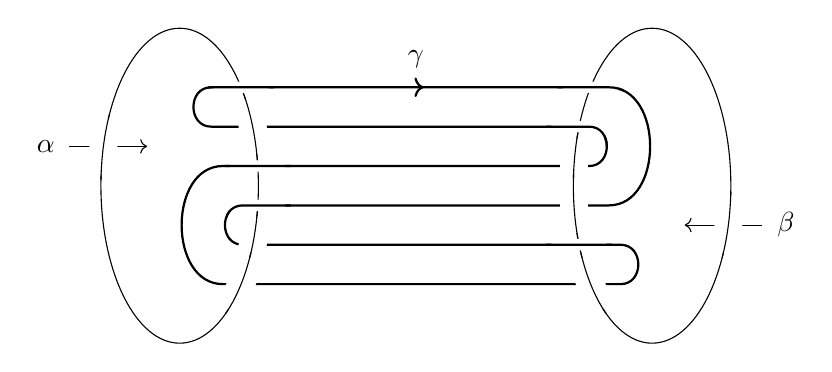
\begin{tikzpicture}
\begin{knot}[clip width = 5, ignore endpoint intersections = false,
%draft mode = crossings]
flip crossing/.list = {1, 2, 8, 10, 4, 12}]
\strand (-3, 0) ellipse (1 and 2);
\strand (3, 0) ellipse (1 and 2);

\strand[thick] 
	(-2.6, 1.25) -- 
	(2.45, 1.25) .. controls +(0.7, 0) and +(0.7, 0) ..
	(2.45, -0.25) --
	(-2.2, -0.25) .. controls +(-0.3, 0) and +(-0.3, 0) ..
	(-2.2, -0.75) --
	(2.6, -0.75) .. controls +(0.3, 0) and +(0.3, 0) ..
	(2.6, -1.25) --
	(-2.45, -1.25) .. controls +(-0.7, 0) and +(-0.7, 0) ..
	(-2.45, 0.25) --
	(2.2, 0.25) .. controls +(0.3, 0) and +(0.3, 0) ..
	(2.2, 0.75) --
	(-2.6, 0.75) .. controls +(-0.3, 0) and +(-0.3, 0) ..
	(-2.6, 1.25);

\strand[->] (-4.4, 0.5) -- (-3.4, 0.5);
\strand[->] (4.4, -0.5) -- (3.4, -0.5);
\end{knot}
\draw[thick, ->] (-1, 1.25) -- (0.1, 1.25);
\node at (-4.7, 0.5) {$\alpha$};
\node at (4.7, -0.5) {$\beta$};
\node at (0, 1.6) {$\gamma$};
\end{tikzpicture}
\caption{The curve $\gamma$, representing the word $\beta^{-1}\alpha^{-1}\beta^{-1}\alpha\beta\alpha$}
\label{fig:the-real-life-gamma}
\end{figure}

Consider the curve $\gamma$ in Figure \ref{fig:the-real-life-gamma}, yielding the single through-slit relation $aba = bab$, which is already in our list of Wirtinger relations.

Finally, the single same-slit relation is $b = b'$, as can be seen by staring at Figure \ref{fig:ribbon-nbhds-of-slits-removed}. This yields the presentation
$$
\pi(R) = \langle a, b, b' \; | \;
aba = bab, ab'a = b'ab', b = b'\rangle = \pi(3_1).$$
\end{example}

\begin{example}[The Knot $8_{20}$]\label{ex:8-20-ribbon}
Consider the following diagram of $K = 8_{20}$. Note that $K$ is also the $(3, -3, 2)$-pretzel knot. It is a so-called ribbon diagram, so it should not be necessary to explicitly draw the ribbon. The knot group $\pi(K)$ is generated by the meridians $a, a', b, b'$ indicated in Figure \ref{fig:ribbon-diagram-of-8_20}.

\begin{figure}[htb]
\centering
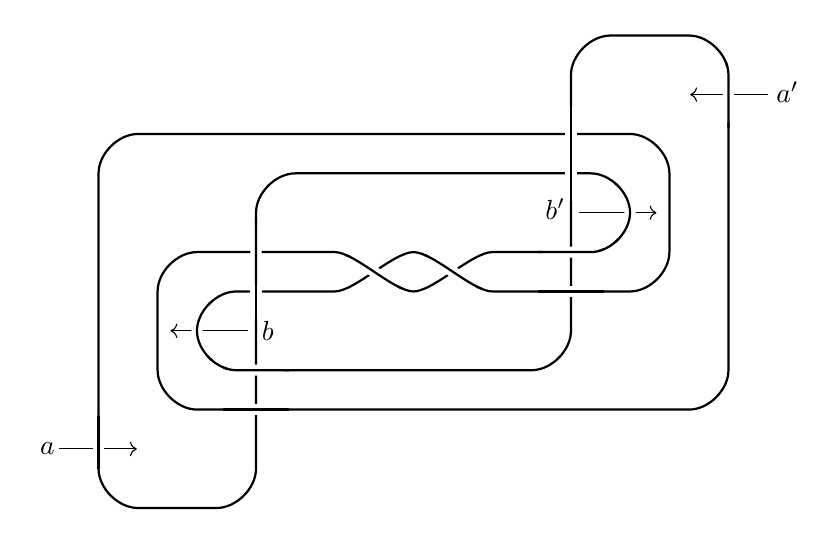
\begin{tikzpicture}
\clip (-4.9, -3.1) rectangle (4.9, 3.1);
\begin{knot}[clip width = 5, consider self intersections=true, ignore endpoint intersections = false,
%draft mode = crossings,
flip crossing/.list = {3, 6, 10, 7, 14}
]
\strand[thick] 
	(-4, -2.5) --
	(-4, 1.25) .. controls +(0, 0.25) and +(-0.25, 0) ..
	(-3.5, 1.75) --
	(2.75, 1.75) .. controls +(0.25, 0) and +(0, 0.25) ..
	(3.25, 1.25) -- 
	(3.25, 0.25) .. controls +(0, -0.25) and +(0.25, 0) ..
	(2.75, -0.25) -- 
	(1, -0.25) .. controls +(-0.25, 0) and +(0.25, 0) ..
	(0, 0.25) .. controls +(-0.25, 0) and +(0.25, 0) ..
	(-1, -0.25) --
	(-2.25, -0.25) .. controls +(-0.25, 0) and +(0, 0.25) ..
	(-2.75, -0.75) .. controls +(0, -0.25) and +(-0.25, 0) ..
	(-2.25, -1.25) --
	(1.5, -1.25) .. controls +(0.25, 0) and +(0, -0.25) ..
	(2, -0.75) --
	(2, 2.5) .. controls +(0, 0.25) and +(-0.25, 0) ..
	(2.5, 3) --
	(3.5, 3) .. controls +(0.25, 0) and +(0, 0.25) ..
	(4, 2.5) -- 
	(4, -1.25) .. controls +(0, -0.25) and +(0.25, 0) ..
	(3.5, -1.75) --
	(-2.75, -1.75) .. controls +(-0.25, 0) and +(0, -0.25) ..
	(-3.25, -1.25) -- 
	(-3.25, -0.25) .. controls +(0, 0.25) and +(-0.25, 0) ..
	(-2.75, 0.25) -- 
	(-1, 0.25) .. controls +(0.25, 0) and +(-0.25, 0) ..
	(0, -0.25) .. controls +(0.25, 0) and +(-0.25, 0) ..
	(1, 0.25) -- 
	(2.25, 0.25) .. controls +(0.25, 0) and +(0, -0.25) ..
	(2.75, 0.75) .. controls +(0, 0.25) and +(0.25, 0) ..
	(2.25, 1.25) -- 
	(-1.5, 1.25) .. controls +(-0.25, 0) and +(0, 0.25) ..
	(-2, 0.75) --
	(-2, -2.5) .. controls +(0, -0.25) and +(0.25, 0) ..
	(-2.5, -3) --
	(-3.5, -3) .. controls +(-0.25, 0) and +(0, -0.25) ..
	(-4, -2.5);
	
\strand[->] (-4.5, -2.25) -- (-3.5, -2.25);
\strand[->] (4.5, 2.25) -- (3.5, 2.25);
\strand[->] (-2.1, -0.75) -- (-3.1, -0.75);
\strand[->] (2.1, 0.75) -- (3.1, 0.75);
\end{knot}
\node at (-4.65, -2.25) {$a$};
\node at (4.75, 2.28) {$a'$};
\node at (-1.85, -0.75) {$b$};
\node at (1.8, 0.8) {$b'$};
\end{tikzpicture}
\caption{A ribbon diagram of $8_{20}$. 
Note that $a$ and $a'$ pass through a ribbon slit, but $b$ and $b'$ do not.}
\label{fig:ribbon-diagram-of-8_20}
\end{figure}

\begin{figure}[htb]
\centering
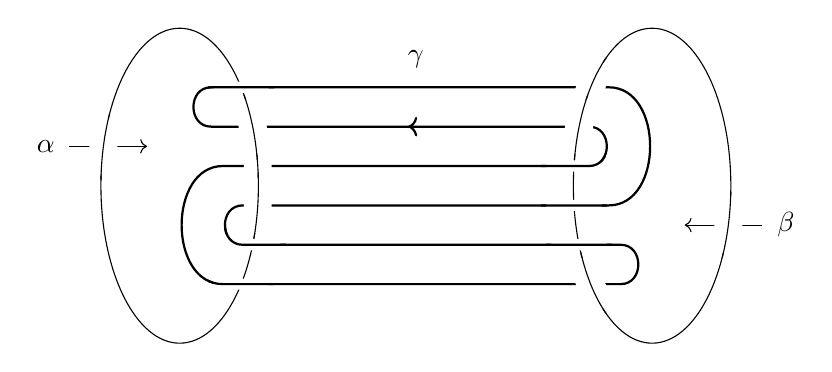
\begin{tikzpicture}
\begin{knot}[clip width = 5, ignore endpoint intersections = false,
%draft mode = crossings]
flip crossing/.list = {1, 9, 11, 12, 5, 6, 12}]
\strand (-3, 0) ellipse (1 and 2);
\strand (3, 0) ellipse (1 and 2);

\strand[thick] 
	(-2.6, 1.25) -- 
	(2.45, 1.25) .. controls +(0.7, 0) and +(0.7, 0) ..
	(2.45, -0.25) --
	(-2.2, -0.25) .. controls +(-0.3, 0) and +(-0.3, 0) ..
	(-2.2, -0.75) --
	(2.6, -0.75) .. controls +(0.3, 0) and +(0.3, 0) ..
	(2.6, -1.25) --
	(-2.45, -1.25) .. controls +(-0.7, 0) and +(-0.7, 0) ..
	(-2.45, 0.25) --
	(2.2, 0.25) .. controls +(0.3, 0) and +(0.3, 0) ..
	(2.2, 0.75) --
	(-2.6, 0.75) .. controls +(-0.3, 0) and +(-0.3, 0) ..
	(-2.6, 1.25);

\strand[->] (-4.4, 0.5) -- (-3.4, 0.5);
\strand[->] (4.4, -0.5) -- (3.4, -0.5);
\end{knot}
\draw[thick, ->] (1, 0.75) -- (-0.1, 0.75);
\node at (-4.7, 0.5) {$\alpha$};
\node at (4.7, -0.5) {$\beta$};
\node at (0, 1.6) {$\gamma$};
\end{tikzpicture}
\caption{The curve $\gamma$ passing through both slits, representing the word $\alpha \beta \alpha \beta^{-1} \alpha^{-1} \beta^{-1}$}
\label{fig:slit-curve-8-20}
\end{figure}

Since $b$ can be arranged to pass through the same slit as $a'$, we add the relation $b = a'$. Moreover, considering the curve $\gamma$ in Figure \ref{fig:slit-curve-8-20}, we see that $a$ and $b$ satisfy the relation $aba = bab$. Finally, after passing under the strand labeled $a'$ we have that $b'$ passes through the same slit as $a$. In symbols, $b' = b^{-1}ab$. Thus we obtain $\pi(R) = \langle a, b \; | \; aba = bab \rangle = \pi(3_1)$.
\end{example}



\begin{theorem}
Let $K$ be any knot and let $R$ be the standard ribbon disk of $K\#\bar{K}$. Then $\pi(R)$ is isomorphic to the knot group $\pi(K)$.
\end{theorem}

\begin{proof}[Proof sketch]
Consider the inclusion $\iota: S^3 \setminus K\#\bar K \rightarrow D^4 \setminus R$. This map induces a surjective homomorphism $\iota_*: \pi(K\#\bar K) \twoheadrightarrow \pi(R)$. Note that sending each meridian in $\pi(K)$ to a meridian of one of the summands in $\pi(K\#\bar K)$ defines an embedding $d: \pi(K) \hookrightarrow \pi(K\#\bar K)$. Composition yields a map 
$$\varphi: \pi(K) \hookrightarrow \pi(K\# \bar K) 
\twoheadrightarrow \pi(R).$$

The homomorphism $\varphi$ is surjective because the image of $d$ together with the kernel of $\iota_*$ generate the knot group $\pi(K\#\bar K)$. Indeed, the same-slit relations are of the form $a^{-1}a'$, where $a$ lies in the image of $d$ and $a'$ is the mirror image of~$a$. For injectivity, we only need to prove that the through-slit relations follow from the Wirtinger relations. To see this, let us change our perspective a little bit. Consider the ribbon disk from the side. This is just a diagram of $K$ where we remove an understrand. For the sideways view of the ribbon disk of the connected sum of the trefoil with its mirror image in Figure \ref{fig:ribbon-trefoil-mirror-trefoil} consider Figure \ref{fig:ribbon-trefoil-from-side}.
Let us refer to a segment of this diagram that starts and ends with overcrossings and only has undercrossings in between as an \textit{anti-bridge}. Then anti-bridges correspond to through-slit relations. Moreover, the qualitative picture of an anti-bridge is as in Figure \ref{fig:anti-bridge}.
In this picture, it is evident that the through-slit relations follow from the Wirtinger relations.
\end{proof}

\begin{figure}[htb]
\centering
\begin{minipage}[b]{0.4\textwidth}
\centering
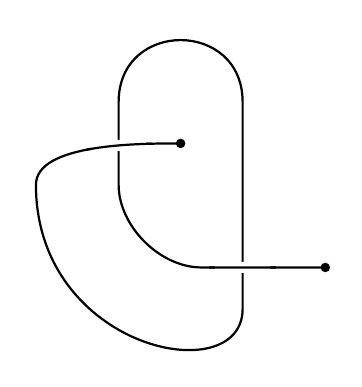
\begin{tikzpicture}[scale = 1.05]
\clip (-1.1, -2.1) rectangle (2.6, 1.9);
\begin{knot}[clip width = 5, consider self intersections = true, ignore endpoint intersections = false, flip crossing = 2
]
\strand[thick] 
	(2.5, -1)  -- 
	(1, -1) .. controls +(-.5, 0) and +(0, -.5) ..
	(0, 0) -- 
	(0, 1) .. controls +(0, 1) and +(0, 1) ..
	(1.5, 1) --
	(1.5, -1.5) .. controls +(0, -1) and +(0, -2) ..
	(-1, 0) .. controls +(0, 0.5) and +(-.5, 0) ..
	(0.75, 0.5);
%\strand[->]
%	(1.3, -0.9)  -- 
%	(1, -0.9) .. controls +(-.4, 0) and +(0, -.4) ..
%	(0.1, 0) -- 
%	(0.1, 1) .. controls +(0, 0.9) and +(0, 0.9) ..
%	(1.4, 1) --
%	(1.4, -1.5) .. controls +(0, -0.85) and +(0, -1.7) ..
%	(-0.9, -0.1) .. controls +(0, 0.4) and +(-.4, 0) ..
%	(-0.1, 0.35);
\end{knot}
\draw[fill = black] (0.75, 0.5) circle (0.05);
\draw[fill = black] (2.5, -1) circle (0.05);
\end{tikzpicture}
\caption{Sideways view of ribbon disk}
\label{fig:ribbon-trefoil-from-side}
\end{minipage}%
\begin{minipage}[b]{0.6\textwidth}
\centering
\begin{tikzpicture}[yscale=1]
\begin{knot}[clip width = 5]

\strand[thick] (2.5, -2) -- (2.5, 2);
\strand[thick] (4, -2) -- (4, 2);
\strand[thick] (5.5, -2) -- (5.5, 2);

\strand[thick] (0, 0) -- (8, 0);

\strand[thick] (1, -2) -- (1, 2);
\strand[thick] (7, -2) -- (7, 2);

\strand[->] (2, 0.75) -- (3, 0.75);
\strand[->] (3.5, 0.75) -- (4.5, 0.75);
\strand[->] (5, 0.75) -- (6, 0.75);
\strand[->] (6, -0.75) -- (5, -0.75);
\strand[->] (4.5, -0.75) -- (3.5, -0.75);
\strand[->] (3, -0.75) -- (2, -0.75);
\strand[->] (1.75, -0.5) -- (1.75, 0.5);
\strand[->] (6.25, 0.5) -- (6.25, -0.5);
\end{knot}
\end{tikzpicture}
\caption{An anti-bridge with $3$ overcrossings}
\label{fig:anti-bridge}
\end{minipage}
\end{figure}

\subsection{Meridians and Ribbons}
Similar as in the case of knots, we have that $H_1(D^4 \setminus D)$ is infinite cyclic for any slice disk $D$. A generator of $H_1(D^4 \setminus D)$ seen as an element of $\pi(D)$ is called a \textit{meridian}. The least number of meridians needed to generate $\pi(D)$ is called the \textit{meridional rank} of $D$, denoted $\mu (D)$. The meridional ranks of the ribbon of the square knot in Example \ref{ex:square-knot-ribbon}, as well as the meridional rank of the ribbon of the knot $8_{20}$ in Example \ref{ex:8-20-ribbon}, were two.

Continuing the analogy, think of a ribbon disk $R$ as an immersed disk in $S^3$. We define its \textit{bridge index} $b(R)$ to be the minimal number of local maxima of a smooth function $S^3 \rightarrow \mathbb{R}$ restricted to ribbons isotopic to $R$. We can now formulate the following.

\begin{conjecture}[Meribbonal Rank Conjecture]
Let $R$ be an immersed ribbon disk in $S^3$. Then the meridional rank of its standard embedding into $D^4$ is equal to its bridge index. In symbols, $$\mu(R) = b(R).$$
\end{conjecture}

One inequality might be doable for me in the near future.

\begin{conjecture}\label{conj:meribbonal-rank-easy}
Let $R$ be any ribbon disk. Then $\mu(R) \leq b(R)$.
\end{conjecture}

\begin{proof}[Proof strategy]
The bridges of ribbon disks are either bridges of the knot or correspond to pairs of bridges which are related by the same-slice relations.
\end{proof}

If Conjecture \ref{conj:meribbonal-rank-easy} were to hold true, we would immediately reduce the meridional rank conjecture to the meribbonal rank conjecture.

\begin{conjecture}
Let $K$ be any knot. Then the standard ribbon for $K \# \bar{K}$ satisfies the meribbonal rank conjecture if and only if $K$ satisfies the meridional rank conjecture.
\end{conjecture}

\begin{proof}[Conditional proof]
The bridge index of the ribbon is the same as the bridge index of $K$, for drawable reasons.
\end{proof}

\subsection{Coxeter Quotients of Ribbon Disks}

A \textit{Coxeter quotient} of a ribbon disk $R$ is a surjection $\pi(R) \rightarrow W$ for some Coxeter group $W$, where meridians of $R \subset D^4$ are mapped to reflections in $W$. Coxeter rank is defined in the obvious way.

\begin{proposition}
Let $R$ be an immersed ribbon disk in $S^3$. Then we have that $c(R) \leq \mu(R)$.
\end{proposition}

\begin{proof}
Note that all knot meridians are also meridians of $D^4$ by including them into the ribbon complement. From here, the proof is completely analogous to what we had before.
\end{proof}

Let $R$ be a ribbon disk. We are now going to consider the reflection quotient $r(R) = \pi(R)^{(2)}$, where relations are added to a presentation of $\pi(R)$ such that each meridian has order two. In this section, we are going to describe a procedure to compute the reflection quotient. On our way to describing this procedure, we will notice some analogies to some notions in knot theory as described in Section \ref{sec:knot-theory}.

We will now think of $R$ as a subset of the four-disk $D^4$. A projection of $R$ onto $S^3$ that only contains (transversal) ribbon singularities will be called a \textit{diagram} of $R$ in this section. Fix a diagram~$E$ of $R$ and let $I$ be the set of singularities of $R$. A connected component of $I$ is a \textit{crossing}, previously also referred to as a ribbon singularity. A connected component of $R \setminus I$ is called an \textit{arc}. Note that for each crossing $C$ of $R$ there are exactly three arcs whose closures meet $C$. The two arcs whose boundaries intersect $C$ are called the \textit{under-arcs} of $C$, and the third arc is called the \textit{over-arc} of $C$. An arc that is an over-arc of at least one crossing is called a \textit{bridge}.

\begin{algo}[Ribbon Wirtinger]\label{alg:ribbon-wirtinger}
Let $R$ be a ribbon disk with diagram $E$. Let $\mathcal{A}$ be the set of arcs of $E$. For each crossing $C$ of $E$, add the relation $ac = cb$ to the set $\mathcal{W}$, where $a, b$ are the under-arcs of $C$ and $c$ is the over-arc of $C$. Then $r(R)$ is isomorphic to the group $\langle \mathcal{A} \; | \; \mathcal{W} \rangle^{(2)}$.
\end{algo}

By taking orientations into account, Procedure \ref{alg:ribbon-wirtinger} could be modified to give another procedure for computing the ribbon group. But this is a little bit over my head so this is left out of this text.

\subsection{Rank Two Quotients}

\begin{question}
In order to check quickly whether a given ribbon admits rank two Coxeter quotients, is there an analogy of the determinant for ribbon disks? What would we like to color?
\end{question}



\newpage

\appendix
\section{Appendix}\label{sec:data}
Table \ref{tab:cox-quotients-10-crossings} consists of the Coxeter quotients we found for $3$-bridge knots of crossing number $10$. It was computed using the same algorithm as in Section \ref{subsec:list-of-quotients}. No quotients were found for $10_{79}, 10_{80}, 10_{81}, 
10_{83}$, $10_{86}$, $10_{88}$, $10_{89}$, $10_{91}$, $10_{92}$, $10_{94}$, $10_{95}$, $10_{96}$, $10_{97}$,
$10_{100}$, $10_{101}$, $10_{103}$, $10_{104}$, $10_{105}$, $10_{106}$, $10_{107}$, $10_{109}$, $10_{110}$, $10_{111}$, $10_{114}$, $10_{115}$, $10_{116}$, $10_{117}$, $10_{118}$, $10_{119}$, $10_{121}$, $10_{122}$, $10_{123}$,
$10_{148}$, $10_{149}$, $10_{150}$, $10_{151}$, $10_{152}$, $10_{153}$, $10_{154}$, $10_{155}$, $10_{156}$, $10_{158}$,
$10_{160}$, $10_{161}$, $10_{162}$ and $10_{163}$. The knots that are not mentioned are $2$-bridge knots.

\begin{table}[htb]
\newcommand{\correctspace}{$\;\;\,$}
\centering
\begin{minipage}[t]{0.5\textwidth}
\centering
\begin{tabular}[t]{c|c}
Knot & Coxeter Quotients \\
\hline
\verticalcenter{$10_{46}$} & \verticalcenter{\coxathreetype{$5$}} \\
\verticalcenter{$10_{47}$} & \verticalcenter{\coxathreetype{$5$}} \\
\verticalcenter{$10_{48}$} & \verticalcenter{\coxathreetype{$5$}} \\
\verticalcenter{$10_{49}$} & \verticalcenter{\coxathreetype{$5$}} \\
\verticalcenter{$10_{50}$} & \verticalcenter{\coxathreetype{$7$}} \\
\verticalcenter{$10_{51}$} & \verticalcenter{\coxathreetype{$7$}} \\
\verticalcenter{$10_{52}$} & \verticalcenter{\coxathreetype{$7$}} \\
\verticalcenter{$10_{53}$} & \verticalcenter{\coxathreetype{$7$}} \\
\verticalcenter{$10_{54}$} & \verticalcenter{\coxathreetype{$7$}} \\
\verticalcenter{$10_{55}$} & \verticalcenter{\coxathreetype{$7$}} \\
\verticalcenter{$10_{56}$} & \verticalcenter{\coxathreetype{$7$}} \\
\verticalcenter{$10_{57}$} & \verticalcenter{\coxathreetype{$7$}} \\
\verticalcenter{$10_{58}$} & \correctspace\verticalcenter{\verticalcenter{\coxathreetype{$5$}} and \verticalcenter{\coxathreetypedouble{$5$}{$5$}}} \\ 
\verticalcenter{$10_{59}$} & \correctspace\verticalcenter{\verticalcenter{\coxathreetype{$5$}} and \verticalcenter{\coxathreetypedouble{$5$}{$5$}}} \\ 
\verticalcenter{$10_{60}$} & \correctspace\verticalcenter{\verticalcenter{\coxathreetype{$5$}} and \verticalcenter{\coxathreetypedouble{$5$}{$5$}}} \\ 
\verticalcenter{$10_{61}$} & \verticalcenter{\coxfourthreethree} \\
\verticalcenter{$10_{62}$} & \verticalcenter{\coxfourthreethree} \\
\verticalcenter{$10_{63}$} & \verticalcenter{\coxfourthreethree} \\
\verticalcenter{$10_{64}$} & \verticalcenter{\coxfourthreethree} \\
\verticalcenter{$10_{65}$} & \verticalcenter{\coxfourthreethree} \\
\verticalcenter{$10_{66}$} & \verticalcenter{\coxfourthreethree} \\
\verticalcenter{$10_{67}$} & \verticalcenter{\verticalcenter{\coxathreetype{$5$}} and \verticalcenter{\coxthreethreethreetype{$5$}}} \\
\verticalcenter{$10_{68}$} & \verticalcenter{\verticalcenter{\coxathreetype{$5$}} and \verticalcenter{\coxthreethreethreetype{$5$}}} \\
\verticalcenter{$10_{69}$} & \verticalcenter{\verticalcenter{\coxathreetype{$5$}} and \verticalcenter{\coxthreethreethreetype{$5$}}} \\
\verticalcenter{$10_{70}$} & \verticalcenter{\coxathreetype{$5$}} \\
\verticalcenter{$10_{71}$} & \verticalcenter{\coxathreetype{$5$}} \\
\verticalcenter{$10_{72}$} & \verticalcenter{\coxathreetype{$5$}} \\
\verticalcenter{$10_{73}$} & \verticalcenter{\coxathreetype{$5$}} \\
\verticalcenter{$10_{76}$} & \verticalcenter{\coxtwothreethree} \\
\verticalcenter{$10_{77}$} & \verticalcenter{\coxtwothreethree} \\
\verticalcenter{$10_{78}$} & \verticalcenter{\coxtwothreethree} \\
\verticalcenter{$10_{82}$} & \verticalcenter{\coxtwothreethree} \\
\verticalcenter{$10_{84}$} & \verticalcenter{\coxtwothreethree} \\
\verticalcenter{$10_{85}$} & \verticalcenter{\coxtwothreethree} \\
\verticalcenter{$10_{87}$} & \verticalcenter{\coxtwothreethree} \\
\verticalcenter{$10_{90}$} & \verticalcenter{\coxathreetype{$5$}} \\
\verticalcenter{$10_{93}$} & \verticalcenter{\coxathreetype{$5$}} \\
\end{tabular}
\end{minipage}%
\begin{minipage}[t]{0.5\textwidth}
\centering
\begin{tabular}[t]{c|c}
Knot & Coxeter Quotients \\
\hline
\verticalcenter{$10_{98}$}\rule{0pt}{4ex} & \verticalcenter{\verticalcenter{\coxathreetype{$5$}} and \verticalcenter{\coxthreethreethreetype{$\infty$}}} \\
\verticalcenter{$10_{99}$} & \verticalcenter{\verticalcenter{\coxathreetype{$5$}} and \verticalcenter{\coxthreethreethreetype{$\infty$}}} \\
\verticalcenter{$10_{102}$} & \verticalcenter{\coxathreetype{$5$}} \\
\verticalcenter{$10_{108}$} & \verticalcenter{\coxathreetype{$5$}} \\
\verticalcenter{$10_{112}$} & \verticalcenter{\coxathreetype{$5$}} \\\verticalcenter{$10_{113}$} & \verticalcenter{\coxathreetype{$5$}} \\
\verticalcenter{$10_{120}$} & \verticalcenter{\coxtwothreethree} \\
\verticalcenter{$10_{124}$} & \verticalcenter{\coxathreetype{$5$}} \\
\verticalcenter{$10_{125}$} & \verticalcenter{\coxathreetype{$5$}} \\
\verticalcenter{$10_{126}$} & \verticalcenter{\coxathreetype{$5$}} \\
\verticalcenter{$10_{127}$} & \verticalcenter{\coxathreetype{$5$}} \\
\verticalcenter{$10_{128}$} & \verticalcenter{\coxathreetype{$7$}} \\
\verticalcenter{$10_{129}$} & \verticalcenter{\coxathreetype{$7$}} \\
\verticalcenter{$10_{130}$} & \verticalcenter{\coxathreetype{$7$}} \\
\verticalcenter{$10_{131}$} & \verticalcenter{\coxathreetype{$7$}} \\
\verticalcenter{$10_{132}$} & \verticalcenter{\coxathreetype{$7$}} \\
\verticalcenter{$10_{133}$} & \verticalcenter{\coxathreetype{$7$}} \\
\verticalcenter{$10_{134}$} & \verticalcenter{\coxathreetype{$7$}} \\
\verticalcenter{$10_{135}$} & \verticalcenter{\coxathreetype{$7$}} \\
\verticalcenter{$10_{136}$} & \correctspace\verticalcenter{\verticalcenter{\coxathreetype{$5$}} and \verticalcenter{\coxathreetypedouble{$5$}{$5$}}} \\
\verticalcenter{$10_{137}$} & \correctspace\verticalcenter{\verticalcenter{\coxathreetype{$5$}} and \verticalcenter{\coxathreetypedouble{$5$}{$5$}}} \\
\verticalcenter{$10_{138}$} & \correctspace\verticalcenter{\verticalcenter{\coxathreetype{$5$}} and \verticalcenter{\coxathreetypedouble{$5$}{$5$}}} \\
\verticalcenter{$10_{139}$} & \verticalcenter{\coxfourthreethree} \\
\verticalcenter{$10_{140}$} & \verticalcenter{\coxfourthreethree} \\
\verticalcenter{$10_{141}$} & \verticalcenter{\coxfourthreethree} \\
\verticalcenter{$10_{142}$} & \verticalcenter{\coxfourthreethree} \\
\verticalcenter{$10_{143}$} & \verticalcenter{\coxfourthreethree} \\
\verticalcenter{$10_{144}$} & \verticalcenter{\coxfourthreethree} \\
\verticalcenter{$10_{145}$} & \verticalcenter{\coxathreetype{$5$}} \\
\verticalcenter{$10_{146}$} & \verticalcenter{\verticalcenter{\coxathreetype{$5$}} and \verticalcenter{\coxthreethreethreetype{$5$}}} \\\verticalcenter{$10_{147}$} & \verticalcenter{\verticalcenter{\coxathreetype{$5$}} and \verticalcenter{\coxthreethreethreetype{$5$}}} \\
\verticalcenter{$10_{157}$} & \verticalcenter{\coxathreetype{$5$}} \\
\verticalcenter{$10_{159}$} & \verticalcenter{\coxathreetype{$5$}} \\
\verticalcenter{$10_{164}$} & \verticalcenter{\coxtwothreethree} \\ \verticalcenter{$10_{165}$} & \verticalcenter{\coxtwothreethree}
\end{tabular}
\end{minipage}
\caption{List of Coxeter knots with bridge index $3$ and crossing number $10$}
\label{tab:cox-quotients-10-crossings}
\end{table}


\newpage

\bibliography{biblio}
\bibliographystyle{plain}

\end{document}